\documentclass[1p]{elsarticle_modified}
%\bibliographystyle{elsarticle-num}

%\usepackage[colorlinks]{hyperref}
%\usepackage{abbrmath_seonhwa} %\Abb, \Ascr, \Acal ,\Abf, \Afrak
\usepackage{amsfonts}
\usepackage{amssymb}
\usepackage{amsmath}
\usepackage{amsthm}
\usepackage{scalefnt}
\usepackage{amsbsy}
\usepackage{kotex}
\usepackage{caption}
\usepackage{subfig}
\usepackage{color}
\usepackage{graphicx}
\usepackage{xcolor} %% white, black, red, green, blue, cyan, magenta, yellow
\usepackage{float}
\usepackage{setspace}
\usepackage{hyperref}

\usepackage{tikz}
\usetikzlibrary{arrows}

\usepackage{multirow}
\usepackage{array} % fixed length table
\usepackage{hhline}

%%%%%%%%%%%%%%%%%%%%%
\makeatletter
\renewcommand*\env@matrix[1][\arraystretch]{%
	\edef\arraystretch{#1}%
	\hskip -\arraycolsep
	\let\@ifnextchar\new@ifnextchar
	\array{*\c@MaxMatrixCols c}}
\makeatother %https://tex.stackexchange.com/questions/14071/how-can-i-increase-the-line-spacing-in-a-matrix
%%%%%%%%%%%%%%%

\usepackage[normalem]{ulem}

\newcommand{\msout}[1]{\ifmmode\text{\sout{\ensuremath{#1}}}\else\sout{#1}\fi}
%SOURCE: \msout is \stkout macro in https://tex.stackexchange.com/questions/20609/strikeout-in-math-mode

\newcommand{\cancel}[1]{
	\ifmmode
	{\color{red}\msout{#1}}
	\else
	{\color{red}\sout{#1}}
	\fi
}

\newcommand{\add}[1]{
	{\color{blue}\uwave{#1}}
}

\newcommand{\replace}[2]{
	\ifmmode
	{\color{red}\msout{#1}}{\color{blue}\uwave{#2}}
	\else
	{\color{red}\sout{#1}}{\color{blue}\uwave{#2}}
	\fi
}

\newcommand{\Sol}{\mathcal{S}} %segment
\newcommand{\D}{D} %diagram
\newcommand{\A}{\mathcal{A}} %arc


%%%%%%%%%%%%%%%%%%%%%%%%%%%%%5 test

\def\sl{\operatorname{\textup{SL}}(2,\Cbb)}
\def\psl{\operatorname{\textup{PSL}}(2,\Cbb)}
\def\quan{\mkern 1mu \triangleright \mkern 1mu}

\theoremstyle{definition}
\newtheorem{thm}{Theorem}[section]
\newtheorem{prop}[thm]{Proposition}
\newtheorem{lem}[thm]{Lemma}
\newtheorem{ques}[thm]{Question}
\newtheorem{cor}[thm]{Corollary}
\newtheorem{defn}[thm]{Definition}
\newtheorem{exam}[thm]{Example}
\newtheorem{rmk}[thm]{Remark}
\newtheorem{alg}[thm]{Algorithm}

\newcommand{\I}{\sqrt{-1}}
\begin{document}

%\begin{frontmatter}
%
%\title{Boundary parabolic representations of knots up to 8 crossings}
%
%%% Group authors per affiliation:
%\author{Yunhi Cho} 
%\address{Department of Mathematics, University of Seoul, Seoul, Korea}
%\ead{yhcho@uos.ac.kr}
%
%
%\author{Seonhwa Kim} %\fnref{s_kim}}
%\address{Center for Geometry and Physics, Institute for Basic Science, Pohang, 37673, Korea}
%\ead{ryeona17@ibs.re.kr}
%
%\author{Hyuk Kim}
%\address{Department of Mathematical Sciences, Seoul National University, Seoul 08826, Korea}
%\ead{hyukkim@snu.ac.kr}
%
%\author{Seokbeom Yoon}
%\address{Department of Mathematical Sciences, Seoul National University, Seoul, 08826,  Korea}
%\ead{sbyoon15@snu.ac.kr}
%
%\begin{abstract}
%We find all boundary parabolic representation of knots up to 8 crossings.
%
%\end{abstract}
%\begin{keyword}
%    \MSC[2010] 57M25 
%\end{keyword}
%
%\end{frontmatter}

%\linenumbers
%\tableofcontents
%
\newcommand\colored[1]{\textcolor{white}{\rule[-0.35ex]{0.8em}{1.4ex}}\kern-0.8em\color{red} #1}%
%\newcommand\colored[1]{\textcolor{white}{ #1}\kern-2.17ex	\textcolor{white}{ #1}\kern-1.81ex	\textcolor{white}{ #1}\kern-2.15ex\color{red}#1	}

{\Large $\underline{12a_{0484}~(K12a_{0484})}$}

\setlength{\tabcolsep}{10pt}
\renewcommand{\arraystretch}{1.6}
\vspace{1cm}\begin{tabular}{m{100pt}>{\centering\arraybackslash}m{274pt}}
\multirow{5}{120pt}{
	\centering
	\includegraphics[width=112pt]{../../../GIT/diagram.site/Diagrams/png/1285_12a_0484.png}\\
\ \ \ A knot diagram\footnotemark}&
\allowdisplaybreaks
\textbf{Linearized knot diagam} \\
\cline{2-2}
 &
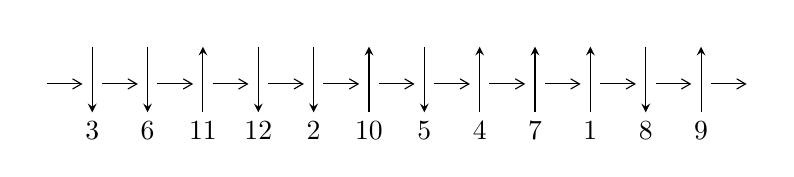
\begin{tikzpicture}[x=20pt, y=17pt]
	% nodes
	\node (C0) at (0, 0) {};
	\node (C1) at (1, 0) {};
	\node (C1U) at (1, +1) {};
	\node (C1D) at (1, -1) {3};

	\node (C2) at (2, 0) {};
	\node (C2U) at (2, +1) {};
	\node (C2D) at (2, -1) {6};

	\node (C3) at (3, 0) {};
	\node (C3U) at (3, +1) {};
	\node (C3D) at (3, -1) {11};

	\node (C4) at (4, 0) {};
	\node (C4U) at (4, +1) {};
	\node (C4D) at (4, -1) {12};

	\node (C5) at (5, 0) {};
	\node (C5U) at (5, +1) {};
	\node (C5D) at (5, -1) {2};

	\node (C6) at (6, 0) {};
	\node (C6U) at (6, +1) {};
	\node (C6D) at (6, -1) {10};

	\node (C7) at (7, 0) {};
	\node (C7U) at (7, +1) {};
	\node (C7D) at (7, -1) {5};

	\node (C8) at (8, 0) {};
	\node (C8U) at (8, +1) {};
	\node (C8D) at (8, -1) {4};

	\node (C9) at (9, 0) {};
	\node (C9U) at (9, +1) {};
	\node (C9D) at (9, -1) {7};

	\node (C10) at (10, 0) {};
	\node (C10U) at (10, +1) {};
	\node (C10D) at (10, -1) {1};

	\node (C11) at (11, 0) {};
	\node (C11U) at (11, +1) {};
	\node (C11D) at (11, -1) {8};

	\node (C12) at (12, 0) {};
	\node (C12U) at (12, +1) {};
	\node (C12D) at (12, -1) {9};
	\node (C13) at (13, 0) {};

	% arrows
	\draw[->,>={angle 60}]
	(C0) edge (C1) (C1) edge (C2) (C2) edge (C3) (C3) edge (C4) (C4) edge (C5) (C5) edge (C6) (C6) edge (C7) (C7) edge (C8) (C8) edge (C9) (C9) edge (C10) (C10) edge (C11) (C11) edge (C12) (C12) edge (C13) ;	\draw[->,>=stealth]
	(C1U) edge (C1D) (C2U) edge (C2D) (C3D) edge (C3U) (C4U) edge (C4D) (C5U) edge (C5D) (C6D) edge (C6U) (C7U) edge (C7D) (C8D) edge (C8U) (C9D) edge (C9U) (C10D) edge (C10U) (C11U) edge (C11D) (C12D) edge (C12U) ;
	\end{tikzpicture} \\
\hhline{~~} \\& 
\textbf{Solving Sequence} \\ \cline{2-2} 
 &
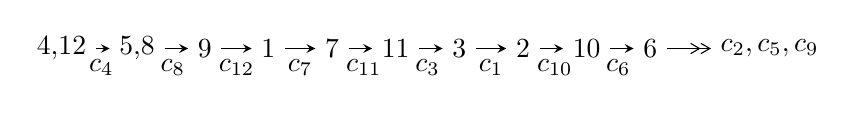
\begin{tikzpicture}[x=23pt, y=7pt]
	% node
	\node (A0) at (-1/8, 0) {4,12};
	\node (A1) at (17/16, 0) {5,8};
	\node (A2) at (17/8, 0) {9};
	\node (A3) at (25/8, 0) {1};
	\node (A4) at (33/8, 0) {7};
	\node (A5) at (41/8, 0) {11};
	\node (A6) at (49/8, 0) {3};
	\node (A7) at (57/8, 0) {2};
	\node (A8) at (65/8, 0) {10};
	\node (A9) at (73/8, 0) {6};
	\node (C1) at (1/2, -1) {$c_{4}$};
	\node (C2) at (13/8, -1) {$c_{8}$};
	\node (C3) at (21/8, -1) {$c_{12}$};
	\node (C4) at (29/8, -1) {$c_{7}$};
	\node (C5) at (37/8, -1) {$c_{11}$};
	\node (C6) at (45/8, -1) {$c_{3}$};
	\node (C7) at (53/8, -1) {$c_{1}$};
	\node (C8) at (61/8, -1) {$c_{10}$};
	\node (C9) at (69/8, -1) {$c_{6}$};
	\node (A10) at (11, 0) {$c_{2},c_{5},c_{9}$};

	% edge
	\draw[->,>=stealth]	
	(A0) edge (A1) (A1) edge (A2) (A2) edge (A3) (A3) edge (A4) (A4) edge (A5) (A5) edge (A6) (A6) edge (A7) (A7) edge (A8) (A8) edge (A9) ;
	\draw[->>,>={angle 60}]	
	(A9) edge (A10);
\end{tikzpicture} \\ 

\end{tabular} \\

\footnotetext{
The image of knot diagram is generated by the software ``\textbf{Draw programme}" developed by Andrew Bartholomew(\url{http://www.layer8.co.uk/maths/draw/index.htm\#Running-draw}), where we modified some parts for our purpose(\url{https://github.com/CATsTAILs/LinksPainter}).
}\phantom \\ \newline 
\centering \textbf{Ideals for irreducible components\footnotemark of $X_{\text{par}}$} 
 
\begin{align*}
I^u_{1}&=\langle 
1.70177\times10^{1756} u^{188}-8.54670\times10^{1756} u^{187}+\cdots+3.45262\times10^{1756} b-4.00960\times10^{1758},\\
\phantom{I^u_{1}}&\phantom{= \langle  }-2.84589\times10^{1758} u^{188}+2.22543\times10^{1759} u^{187}+\cdots+5.00630\times10^{1757} a+6.93573\times10^{1759},\\
\phantom{I^u_{1}}&\phantom{= \langle  }u^{189}-8 u^{188}+\cdots-79 u-29\rangle \\
I^u_{2}&=\langle 
2.30944\times10^{46} u^{38}+1.17665\times10^{46} u^{37}+\cdots+3.78715\times10^{46} b+5.05705\times10^{46},\\
\phantom{I^u_{2}}&\phantom{= \langle  }5.02111\times10^{46} u^{38}-2.41670\times10^{45} u^{37}+\cdots+3.78715\times10^{46} a+1.92218\times10^{46},\;u^{39}+2 u^{37}+\cdots+u+1\rangle \\
I^u_{3}&=\langle 
u^2+b+u-1,\;a,\;u^3- u+1\rangle \\
I^u_{4}&=\langle 
b^3+b^2-1,\;a,\;u+1\rangle \\
\\
\end{align*}
\raggedright * 4 irreducible components of $\dim_{\mathbb{C}}=0$, with total 234 representations.\\
\footnotetext{All coefficients of polynomials are rational numbers. But the coefficients are sometimes approximated in decimal forms when there is not enough margin.}
\newpage
\renewcommand{\arraystretch}{1}
\centering \section*{I. $I^u_{1}= \langle 1.70\times10^{1756} u^{188}-8.55\times10^{1756} u^{187}+\cdots+3.45\times10^{1756} b-4.01\times10^{1758},\;-2.85\times10^{1758} u^{188}+2.23\times10^{1759} u^{187}+\cdots+5.01\times10^{1757} a+6.94\times10^{1759},\;u^{189}-8 u^{188}+\cdots-79 u-29 \rangle$}
\flushleft \textbf{(i) Arc colorings}\\
\begin{tabular}{m{7pt} m{180pt} m{7pt} m{180pt} }
\flushright $a_{4}=$&$\begin{pmatrix}1\\0\end{pmatrix}$ \\
\flushright $a_{12}=$&$\begin{pmatrix}0\\u\end{pmatrix}$ \\
\flushright $a_{5}=$&$\begin{pmatrix}1\\u^2\end{pmatrix}$ \\
\flushright $a_{8}=$&$\begin{pmatrix}5.68461 u^{188}-44.4526 u^{187}+\cdots-782.014 u-138.540\\-0.492894 u^{188}+2.47542 u^{187}+\cdots+328.895 u+116.132\end{pmatrix}$ \\
\flushright $a_{9}=$&$\begin{pmatrix}5.19172 u^{188}-41.9771 u^{187}+\cdots-453.119 u-22.4081\\-0.492894 u^{188}+2.47542 u^{187}+\cdots+328.895 u+116.132\end{pmatrix}$ \\
\flushright $a_{1}=$&$\begin{pmatrix}-3.36772 u^{188}+24.7145 u^{187}+\cdots+813.429 u+190.147\\-0.111564 u^{188}+0.839054 u^{187}+\cdots+75.0790 u+16.1404\end{pmatrix}$ \\
\flushright $a_{7}=$&$\begin{pmatrix}7.22709 u^{188}-58.0830 u^{187}+\cdots-698.897 u-52.1145\\-0.907974 u^{188}+6.31775 u^{187}+\cdots+271.671 u+78.7054\end{pmatrix}$ \\
\flushright $a_{11}=$&$\begin{pmatrix}-4.34178 u^{188}+31.5260 u^{187}+\cdots+999.331 u+256.114\\1.08563 u^{188}-7.65047 u^{187}+\cdots-258.981 u-82.1081\end{pmatrix}$ \\
\flushright $a_{3}=$&$\begin{pmatrix}1.65724 u^{188}-20.1512 u^{187}+\cdots+1296.54 u+598.469\\-2.22531 u^{188}+19.0249 u^{187}+\cdots-28.9240 u-81.4809\end{pmatrix}$ \\
\flushright $a_{2}=$&$\begin{pmatrix}4.14978 u^{188}-30.7763 u^{187}+\cdots-957.636 u-228.563\\-0.462116 u^{188}+3.85116 u^{187}+\cdots+36.8251 u-0.364084\end{pmatrix}$ \\
\flushright $a_{10}=$&$\begin{pmatrix}-3.72955 u^{188}+30.1501 u^{187}+\cdots+400.274 u-12.8958\\0.450649 u^{188}-3.76241 u^{187}+\cdots+7.56524 u+13.0644\end{pmatrix}$ \\
\flushright $a_{6}=$&$\begin{pmatrix}11.1729 u^{188}-89.7928 u^{187}+\cdots-927.699 u-30.6737\\-1.81023 u^{188}+13.7963 u^{187}+\cdots+331.685 u+69.5307\end{pmatrix}$\\&\end{tabular}
\flushleft \textbf{(ii) Obstruction class $= -1$}\\~\\
\flushleft \textbf{(iii) Cusp Shapes $= 12.0861 u^{188}-100.517 u^{187}+\cdots-741.562 u+82.8947$}\\~\\
\newpage\renewcommand{\arraystretch}{1}
\flushleft \textbf{(iv) u-Polynomials at the component}\newline \\
\begin{tabular}{m{50pt}|m{274pt}}
Crossings & \hspace{64pt}u-Polynomials at each crossing \\
\hline $$\begin{aligned}c_{1}\end{aligned}$$&$\begin{aligned}
&u^{189}+86 u^{188}+\cdots+12226241 u+339889
\end{aligned}$\\
\hline $$\begin{aligned}c_{2},c_{5}\end{aligned}$$&$\begin{aligned}
&u^{189}-43 u^{187}+\cdots-6703 u+583
\end{aligned}$\\
\hline $$\begin{aligned}c_{3}\end{aligned}$$&$\begin{aligned}
&u^{189}+4 u^{188}+\cdots+60188019890 u+5986213211
\end{aligned}$\\
\hline $$\begin{aligned}c_{4}\end{aligned}$$&$\begin{aligned}
&u^{189}+8 u^{188}+\cdots-79 u+29
\end{aligned}$\\
\hline $$\begin{aligned}c_{6},c_{9}\end{aligned}$$&$\begin{aligned}
&u^{189}-8 u^{188}+\cdots+54826 u+4031
\end{aligned}$\\
\hline $$\begin{aligned}c_{7}\end{aligned}$$&$\begin{aligned}
&u^{189}-8 u^{188}+\cdots+204513953 u+32543267
\end{aligned}$\\
\hline $$\begin{aligned}c_{8}\end{aligned}$$&$\begin{aligned}
&u^{189}-3 u^{188}+\cdots-26 u+1
\end{aligned}$\\
\hline $$\begin{aligned}c_{10}\end{aligned}$$&$\begin{aligned}
&u^{189}-6 u^{188}+\cdots-47525 u+32287
\end{aligned}$\\
\hline $$\begin{aligned}c_{11}\end{aligned}$$&$\begin{aligned}
&u^{189}+10 u^{188}+\cdots+2304 u-704
\end{aligned}$\\
\hline $$\begin{aligned}c_{12}\end{aligned}$$&$\begin{aligned}
&u^{189}+u^{188}+\cdots+46221377 u+1765261
\end{aligned}$\\
\hline
\end{tabular}\\~\\
\newpage\renewcommand{\arraystretch}{1}
\flushleft \textbf{(v) Riley Polynomials at the component}\newline \\
\begin{tabular}{m{50pt}|m{274pt}}
Crossings & \hspace{64pt}Riley Polynomials at each crossing \\
\hline $$\begin{aligned}c_{1}\end{aligned}$$&$\begin{aligned}
&y^{189}+50 y^{188}+\cdots-10262219485735 y-115524532321
\end{aligned}$\\
\hline $$\begin{aligned}c_{2},c_{5}\end{aligned}$$&$\begin{aligned}
&y^{189}-86 y^{188}+\cdots+12226241 y-339889
\end{aligned}$\\
\hline $$\begin{aligned}c_{3}\end{aligned}$$&$\begin{aligned}
&y^{189}-102 y^{188}+\cdots+3.80\times10^{21} y-3.58\times10^{19}
\end{aligned}$\\
\hline $$\begin{aligned}c_{4}\end{aligned}$$&$\begin{aligned}
&y^{189}+12 y^{188}+\cdots-80179 y-841
\end{aligned}$\\
\hline $$\begin{aligned}c_{6},c_{9}\end{aligned}$$&$\begin{aligned}
&y^{189}+124 y^{188}+\cdots+2605740968 y-16248961
\end{aligned}$\\
\hline $$\begin{aligned}c_{7}\end{aligned}$$&$\begin{aligned}
&y^{189}+62 y^{188}+\cdots-276984664046356039 y-1059064227033289
\end{aligned}$\\
\hline $$\begin{aligned}c_{8}\end{aligned}$$&$\begin{aligned}
&y^{189}-33 y^{188}+\cdots-54 y-1
\end{aligned}$\\
\hline $$\begin{aligned}c_{10}\end{aligned}$$&$\begin{aligned}
&y^{189}-28 y^{188}+\cdots+280760605113 y-1042450369
\end{aligned}$\\
\hline $$\begin{aligned}c_{11}\end{aligned}$$&$\begin{aligned}
&y^{189}+40 y^{188}+\cdots-25982976 y-495616
\end{aligned}$\\
\hline $$\begin{aligned}c_{12}\end{aligned}$$&$\begin{aligned}
&y^{189}-31 y^{188}+\cdots+793233634931023 y-3116146398121
\end{aligned}$\\
\hline
\end{tabular}\\~\\
\newpage\flushleft \textbf{(vi) Complex Volumes and Cusp Shapes}
$$\begin{array}{c|c|c}  
\text{Solutions to }I^u_{1}& \I (\text{vol} + \sqrt{-1}CS) & \text{Cusp shape}\\
 \hline 
\begin{aligned}
u &= \phantom{-}0.844132 + 0.532140 I \\
a &= \phantom{-}1.367490 - 0.140585 I \\
b &= -0.082072 + 0.219551 I\end{aligned}
 & -3.27061 - 6.93518 I & \phantom{-0.000000 } 0 \\ \hline\begin{aligned}
u &= \phantom{-}0.844132 - 0.532140 I \\
a &= \phantom{-}1.367490 + 0.140585 I \\
b &= -0.082072 - 0.219551 I\end{aligned}
 & -3.27061 + 6.93518 I & \phantom{-0.000000 } 0 \\ \hline\begin{aligned}
u &= \phantom{-}0.077394 + 0.992560 I \\
a &= \phantom{-}0.167460 + 1.027600 I \\
b &= -0.147882 - 0.006886 I\end{aligned}
 & \phantom{-}1.67076 - 2.02837 I & \phantom{-0.000000 } 0 \\ \hline\begin{aligned}
u &= \phantom{-}0.077394 - 0.992560 I \\
a &= \phantom{-}0.167460 - 1.027600 I \\
b &= -0.147882 + 0.006886 I\end{aligned}
 & \phantom{-}1.67076 + 2.02837 I & \phantom{-0.000000 } 0 \\ \hline\begin{aligned}
u &= \phantom{-}0.524312 + 0.826486 I \\
a &= \phantom{-}1.75584 - 0.14496 I \\
b &= -1.24305 + 1.02209 I\end{aligned}
 & -1.60540 - 7.04570 I & \phantom{-0.000000 } 0 \\ \hline\begin{aligned}
u &= \phantom{-}0.524312 - 0.826486 I \\
a &= \phantom{-}1.75584 + 0.14496 I \\
b &= -1.24305 - 1.02209 I\end{aligned}
 & -1.60540 + 7.04570 I & \phantom{-0.000000 } 0 \\ \hline\begin{aligned}
u &= -0.441435 + 0.870709 I \\
a &= -1.86746 - 0.44683 I \\
b &= \phantom{-}0.618269 + 0.467411 I\end{aligned}
 & \phantom{-}2.98882 + 7.55128 I & \phantom{-0.000000 } 0 \\ \hline\begin{aligned}
u &= -0.441435 - 0.870709 I \\
a &= -1.86746 + 0.44683 I \\
b &= \phantom{-}0.618269 - 0.467411 I\end{aligned}
 & \phantom{-}2.98882 - 7.55128 I & \phantom{-0.000000 } 0 \\ \hline\begin{aligned}
u &= \phantom{-}0.438106 + 0.925981 I \\
a &= \phantom{-}1.73462 - 0.26957 I \\
b &= -0.666435 + 0.470472 I\end{aligned}
 & \phantom{-}3.77987 - 2.03293 I & \phantom{-0.000000 } 0 \\ \hline\begin{aligned}
u &= \phantom{-}0.438106 - 0.925981 I \\
a &= \phantom{-}1.73462 + 0.26957 I \\
b &= -0.666435 - 0.470472 I\end{aligned}
 & \phantom{-}3.77987 + 2.03293 I & \phantom{-0.000000 } 0\\
 \hline 
 \end{array}$$\newpage$$\begin{array}{c|c|c}  
\text{Solutions to }I^u_{1}& \I (\text{vol} + \sqrt{-1}CS) & \text{Cusp shape}\\
 \hline 
\begin{aligned}
u &= -0.972403 + 0.329413 I \\
a &= \phantom{-}0.255873 + 0.228769 I \\
b &= -0.797104 - 1.119670 I\end{aligned}
 & -2.96973 + 5.60185 I & \phantom{-0.000000 } 0 \\ \hline\begin{aligned}
u &= -0.972403 - 0.329413 I \\
a &= \phantom{-}0.255873 - 0.228769 I \\
b &= -0.797104 + 1.119670 I\end{aligned}
 & -2.96973 - 5.60185 I & \phantom{-0.000000 } 0 \\ \hline\begin{aligned}
u &= \phantom{-}0.961003 + 0.375663 I \\
a &= -0.383816 + 0.060999 I \\
b &= \phantom{-}0.781064 - 0.964056 I\end{aligned}
 & -2.22675 - 1.38549 I & \phantom{-0.000000 } 0 \\ \hline\begin{aligned}
u &= \phantom{-}0.961003 - 0.375663 I \\
a &= -0.383816 - 0.060999 I \\
b &= \phantom{-}0.781064 + 0.964056 I\end{aligned}
 & -2.22675 + 1.38549 I & \phantom{-0.000000 } 0 \\ \hline\begin{aligned}
u &= -0.463199 + 0.846971 I \\
a &= \phantom{-}0.454457 - 0.347296 I \\
b &= -0.583755 + 1.177940 I\end{aligned}
 & \phantom{-}2.97669 - 3.14052 I & \phantom{-0.000000 } 0 \\ \hline\begin{aligned}
u &= -0.463199 - 0.846971 I \\
a &= \phantom{-}0.454457 + 0.347296 I \\
b &= -0.583755 - 1.177940 I\end{aligned}
 & \phantom{-}2.97669 + 3.14052 I & \phantom{-0.000000 } 0 \\ \hline\begin{aligned}
u &= \phantom{-}0.592075 + 0.857434 I \\
a &= \phantom{-}1.48918 - 0.32631 I \\
b &= -1.11116 + 1.04655 I\end{aligned}
 & -1.96159 - 2.07286 I & \phantom{-0.000000 } 0 \\ \hline\begin{aligned}
u &= \phantom{-}0.592075 - 0.857434 I \\
a &= \phantom{-}1.48918 + 0.32631 I \\
b &= -1.11116 - 1.04655 I\end{aligned}
 & -1.96159 + 2.07286 I & \phantom{-0.000000 } 0 \\ \hline\begin{aligned}
u &= -0.935869 + 0.465004 I \\
a &= -1.114220 + 0.027624 I \\
b &= \phantom{-}1.44762 + 0.78090 I\end{aligned}
 & -1.03319 + 5.83684 I & \phantom{-0.000000 } 0 \\ \hline\begin{aligned}
u &= -0.935869 - 0.465004 I \\
a &= -1.114220 - 0.027624 I \\
b &= \phantom{-}1.44762 - 0.78090 I\end{aligned}
 & -1.03319 - 5.83684 I & \phantom{-0.000000 } 0\\
 \hline 
 \end{array}$$\newpage$$\begin{array}{c|c|c}  
\text{Solutions to }I^u_{1}& \I (\text{vol} + \sqrt{-1}CS) & \text{Cusp shape}\\
 \hline 
\begin{aligned}
u &= \phantom{-}0.255882 + 1.027360 I \\
a &= -0.752980 + 0.237470 I \\
b &= \phantom{-}1.21569 - 1.14741 I\end{aligned}
 & \phantom{-}2.14568 - 8.64009 I & \phantom{-0.000000 } 0 \\ \hline\begin{aligned}
u &= \phantom{-}0.255882 - 1.027360 I \\
a &= -0.752980 - 0.237470 I \\
b &= \phantom{-}1.21569 + 1.14741 I\end{aligned}
 & \phantom{-}2.14568 + 8.64009 I & \phantom{-0.000000 } 0 \\ \hline\begin{aligned}
u &= -0.909427 + 0.242629 I \\
a &= -0.092777 + 0.264208 I \\
b &= -0.603081 - 1.219320 I\end{aligned}
 & -3.56617 + 0.88904 I & \phantom{-0.000000 } 0 \\ \hline\begin{aligned}
u &= -0.909427 - 0.242629 I \\
a &= -0.092777 - 0.264208 I \\
b &= -0.603081 + 1.219320 I\end{aligned}
 & -3.56617 - 0.88904 I & \phantom{-0.000000 } 0 \\ \hline\begin{aligned}
u &= -0.760735 + 0.741973 I \\
a &= -1.269530 - 0.033212 I \\
b &= \phantom{-}1.20647 + 0.85554 I\end{aligned}
 & -0.93550 + 5.08812 I & \phantom{-0.000000 } 0 \\ \hline\begin{aligned}
u &= -0.760735 - 0.741973 I \\
a &= -1.269530 + 0.033212 I \\
b &= \phantom{-}1.20647 - 0.85554 I\end{aligned}
 & -0.93550 - 5.08812 I & \phantom{-0.000000 } 0 \\ \hline\begin{aligned}
u &= \phantom{-}1.024840 + 0.334092 I \\
a &= \phantom{-}1.061180 - 0.010190 I \\
b &= -1.55032 + 0.71913 I\end{aligned}
 & -2.78237 - 10.75200 I & \phantom{-0.000000 } 0 \\ \hline\begin{aligned}
u &= \phantom{-}1.024840 - 0.334092 I \\
a &= \phantom{-}1.061180 + 0.010190 I \\
b &= -1.55032 - 0.71913 I\end{aligned}
 & -2.78237 + 10.75200 I & \phantom{-0.000000 } 0 \\ \hline\begin{aligned}
u &= -0.481971 + 0.785729 I \\
a &= -1.78773 + 0.03819 I \\
b &= \phantom{-}1.24712 + 0.96515 I\end{aligned}
 & -1.12829 + 3.14613 I & \phantom{-0.000000 } 0 \\ \hline\begin{aligned}
u &= -0.481971 - 0.785729 I \\
a &= -1.78773 - 0.03819 I \\
b &= \phantom{-}1.24712 - 0.96515 I\end{aligned}
 & -1.12829 - 3.14613 I & \phantom{-0.000000 } 0\\
 \hline 
 \end{array}$$\newpage$$\begin{array}{c|c|c}  
\text{Solutions to }I^u_{1}& \I (\text{vol} + \sqrt{-1}CS) & \text{Cusp shape}\\
 \hline 
\begin{aligned}
u &= \phantom{-}0.404919 + 0.797425 I \\
a &= -0.577919 - 0.289557 I \\
b &= \phantom{-}0.85399 + 1.19964 I\end{aligned}
 & \phantom{-}4.06193 - 2.39062 I & \phantom{-0.000000 } 0 \\ \hline\begin{aligned}
u &= \phantom{-}0.404919 - 0.797425 I \\
a &= -0.577919 + 0.289557 I \\
b &= \phantom{-}0.85399 - 1.19964 I\end{aligned}
 & \phantom{-}4.06193 + 2.39062 I & \phantom{-0.000000 } 0 \\ \hline\begin{aligned}
u &= -0.816150 + 0.344293 I \\
a &= \phantom{-}1.77048 - 1.32209 I \\
b &= -0.400733 - 0.862039 I\end{aligned}
 & -1.93309 + 11.59360 I & \phantom{-0.000000 } 0 \\ \hline\begin{aligned}
u &= -0.816150 - 0.344293 I \\
a &= \phantom{-}1.77048 + 1.32209 I \\
b &= -0.400733 + 0.862039 I\end{aligned}
 & -1.93309 - 11.59360 I & \phantom{-0.000000 } 0 \\ \hline\begin{aligned}
u &= \phantom{-}0.394173 + 1.050300 I \\
a &= \phantom{-}0.362217 + 1.161710 I \\
b &= -0.505060 - 0.119546 I\end{aligned}
 & \phantom{-}2.05531 + 2.16455 I & \phantom{-0.000000 } 0 \\ \hline\begin{aligned}
u &= \phantom{-}0.394173 - 1.050300 I \\
a &= \phantom{-}0.362217 - 1.161710 I \\
b &= -0.505060 + 0.119546 I\end{aligned}
 & \phantom{-}2.05531 - 2.16455 I & \phantom{-0.000000 } 0 \\ \hline\begin{aligned}
u &= \phantom{-}0.852184 + 0.201220 I \\
a &= -1.26967 - 1.84751 I \\
b &= \phantom{-}0.267026 - 0.882857 I\end{aligned}
 & \phantom{-}0.21583 - 5.10553 I & \phantom{-0.000000 } 0 \\ \hline\begin{aligned}
u &= \phantom{-}0.852184 - 0.201220 I \\
a &= -1.26967 + 1.84751 I \\
b &= \phantom{-}0.267026 + 0.882857 I\end{aligned}
 & \phantom{-}0.21583 + 5.10553 I & \phantom{-0.000000 } 0 \\ \hline\begin{aligned}
u &= -0.563946 + 0.980423 I \\
a &= -1.077420 - 0.483235 I \\
b &= \phantom{-}0.831708 + 0.998947 I\end{aligned}
 & -1.88915 + 5.05174 I & \phantom{-0.000000 } 0 \\ \hline\begin{aligned}
u &= -0.563946 - 0.980423 I \\
a &= -1.077420 + 0.483235 I \\
b &= \phantom{-}0.831708 - 0.998947 I\end{aligned}
 & -1.88915 - 5.05174 I & \phantom{-0.000000 } 0\\
 \hline 
 \end{array}$$\newpage$$\begin{array}{c|c|c}  
\text{Solutions to }I^u_{1}& \I (\text{vol} + \sqrt{-1}CS) & \text{Cusp shape}\\
 \hline 
\begin{aligned}
u &= -0.231199 + 0.836142 I \\
a &= \phantom{-}0.876289 + 0.187217 I \\
b &= -1.32730 - 1.19266 I\end{aligned}
 & \phantom{-}4.62208 + 3.22300 I & \phantom{-0.000000 } 0 \\ \hline\begin{aligned}
u &= -0.231199 - 0.836142 I \\
a &= \phantom{-}0.876289 - 0.187217 I \\
b &= -1.32730 + 1.19266 I\end{aligned}
 & \phantom{-}4.62208 - 3.22300 I & \phantom{-0.000000 } 0 \\ \hline\begin{aligned}
u &= -1.010300 + 0.515302 I \\
a &= \phantom{-}0.963300 - 0.276561 I \\
b &= -0.538426 - 0.958597 I\end{aligned}
 & -8.79744 + 2.92392 I & \phantom{-0.000000 } 0 \\ \hline\begin{aligned}
u &= -1.010300 - 0.515302 I \\
a &= \phantom{-}0.963300 + 0.276561 I \\
b &= -0.538426 + 0.958597 I\end{aligned}
 & -8.79744 - 2.92392 I & \phantom{-0.000000 } 0 \\ \hline\begin{aligned}
u &= \phantom{-}0.812549 + 0.223532 I \\
a &= \phantom{-}0.364062 + 0.113016 I \\
b &= \phantom{-}0.451133 - 1.162430 I\end{aligned}
 & -3.49480 - 4.44374 I & \phantom{-0.000000 } 0 \\ \hline\begin{aligned}
u &= \phantom{-}0.812549 - 0.223532 I \\
a &= \phantom{-}0.364062 - 0.113016 I \\
b &= \phantom{-}0.451133 + 1.162430 I\end{aligned}
 & -3.49480 + 4.44374 I & \phantom{-0.000000 } 0 \\ \hline\begin{aligned}
u &= \phantom{-}1.050640 + 0.485882 I \\
a &= -0.772908 - 0.040764 I \\
b &= \phantom{-}0.537958 - 0.866296 I\end{aligned}
 & -3.95762 - 0.09851 I & \phantom{-0.000000 } 0 \\ \hline\begin{aligned}
u &= \phantom{-}1.050640 - 0.485882 I \\
a &= -0.772908 + 0.040764 I \\
b &= \phantom{-}0.537958 + 0.866296 I\end{aligned}
 & -3.95762 + 0.09851 I & \phantom{-0.000000 } 0 \\ \hline\begin{aligned}
u &= -0.483455 + 0.675596 I \\
a &= -1.70770 - 0.53072 I \\
b &= \phantom{-}0.538001 + 0.232331 I\end{aligned}
 & -0.74435 + 3.34325 I & \phantom{-0.000000 } 0 \\ \hline\begin{aligned}
u &= -0.483455 - 0.675596 I \\
a &= -1.70770 + 0.53072 I \\
b &= \phantom{-}0.538001 - 0.232331 I\end{aligned}
 & -0.74435 - 3.34325 I & \phantom{-0.000000 } 0\\
 \hline 
 \end{array}$$\newpage$$\begin{array}{c|c|c}  
\text{Solutions to }I^u_{1}& \I (\text{vol} + \sqrt{-1}CS) & \text{Cusp shape}\\
 \hline 
\begin{aligned}
u &= -0.524063 + 1.064440 I \\
a &= -0.402397 + 1.064550 I \\
b &= \phantom{-}0.606440 - 0.082251 I\end{aligned}
 & \phantom{-}2.32165 + 1.90131 I & \phantom{-0.000000 } 0 \\ \hline\begin{aligned}
u &= -0.524063 - 1.064440 I \\
a &= -0.402397 - 1.064550 I \\
b &= \phantom{-}0.606440 + 0.082251 I\end{aligned}
 & \phantom{-}2.32165 - 1.90131 I & \phantom{-0.000000 } 0 \\ \hline\begin{aligned}
u &= -1.074810 + 0.523504 I \\
a &= \phantom{-}0.874974 + 0.057224 I \\
b &= -0.473977 - 0.886927 I\end{aligned}
 & -6.14757 - 4.91011 I & \phantom{-0.000000 } 0 \\ \hline\begin{aligned}
u &= -1.074810 - 0.523504 I \\
a &= \phantom{-}0.874974 - 0.057224 I \\
b &= -0.473977 + 0.886927 I\end{aligned}
 & -6.14757 + 4.91011 I & \phantom{-0.000000 } 0 \\ \hline\begin{aligned}
u &= \phantom{-}1.243220 + 0.004215 I \\
a &= \phantom{-}0.553465 + 0.552475 I \\
b &= \phantom{-}0.208318 + 0.147278 I\end{aligned}
 & -5.02031 + 1.15207 I & \phantom{-0.000000 } 0 \\ \hline\begin{aligned}
u &= \phantom{-}1.243220 - 0.004215 I \\
a &= \phantom{-}0.553465 - 0.552475 I \\
b &= \phantom{-}0.208318 - 0.147278 I\end{aligned}
 & -5.02031 - 1.15207 I & \phantom{-0.000000 } 0 \\ \hline\begin{aligned}
u &= \phantom{-}0.721507 + 0.226432 I \\
a &= \phantom{-}0.951470 + 0.153049 I \\
b &= -1.68227 + 1.00752 I\end{aligned}
 & -5.37364 - 3.67245 I & \phantom{-0.000000 } 0 \\ \hline\begin{aligned}
u &= \phantom{-}0.721507 - 0.226432 I \\
a &= \phantom{-}0.951470 - 0.153049 I \\
b &= -1.68227 - 1.00752 I\end{aligned}
 & -5.37364 + 3.67245 I & \phantom{-0.000000 } 0 \\ \hline\begin{aligned}
u &= -0.335489 + 1.198390 I \\
a &= -0.484398 - 0.607342 I \\
b &= \phantom{-}0.395175 + 0.966399 I\end{aligned}
 & -1.82265 - 1.07337 I & \phantom{-0.000000 } 0 \\ \hline\begin{aligned}
u &= -0.335489 - 1.198390 I \\
a &= -0.484398 + 0.607342 I \\
b &= \phantom{-}0.395175 - 0.966399 I\end{aligned}
 & -1.82265 + 1.07337 I & \phantom{-0.000000 } 0\\
 \hline 
 \end{array}$$\newpage$$\begin{array}{c|c|c}  
\text{Solutions to }I^u_{1}& \I (\text{vol} + \sqrt{-1}CS) & \text{Cusp shape}\\
 \hline 
\begin{aligned}
u &= -0.266710 + 0.681834 I \\
a &= -1.94690 + 0.63885 I \\
b &= \phantom{-}1.050420 + 0.762270 I\end{aligned}
 & \phantom{-}0.43756 + 6.91669 I & \phantom{-0.000000 } 0 \\ \hline\begin{aligned}
u &= -0.266710 - 0.681834 I \\
a &= -1.94690 - 0.63885 I \\
b &= \phantom{-}1.050420 - 0.762270 I\end{aligned}
 & \phantom{-}0.43756 - 6.91669 I & \phantom{-0.000000 } 0 \\ \hline\begin{aligned}
u &= \phantom{-}0.489581 + 0.517741 I \\
a &= \phantom{-}0.18796 - 1.81514 I \\
b &= \phantom{-}0.493139 - 0.510698 I\end{aligned}
 & -4.38188 - 5.01571 I & \phantom{-0.000000 } 0 \\ \hline\begin{aligned}
u &= \phantom{-}0.489581 - 0.517741 I \\
a &= \phantom{-}0.18796 + 1.81514 I \\
b &= \phantom{-}0.493139 + 0.510698 I\end{aligned}
 & -4.38188 + 5.01571 I & \phantom{-0.000000 } 0 \\ \hline\begin{aligned}
u &= \phantom{-}0.087711 + 0.685167 I \\
a &= \phantom{-}1.30233 - 0.56725 I \\
b &= -0.558581 + 0.531308 I\end{aligned}
 & \phantom{-}0.39710 - 1.51746 I & \phantom{-0.000000 } 0 \\ \hline\begin{aligned}
u &= \phantom{-}0.087711 - 0.685167 I \\
a &= \phantom{-}1.30233 + 0.56725 I \\
b &= -0.558581 - 0.531308 I\end{aligned}
 & \phantom{-}0.39710 + 1.51746 I & \phantom{-0.000000 } 0 \\ \hline\begin{aligned}
u &= \phantom{-}0.317614 + 0.610850 I \\
a &= -0.881266 - 0.165362 I \\
b &= \phantom{-}1.25700 + 1.54157 I\end{aligned}
 & \phantom{-}2.59339 - 6.52868 I & \phantom{-0.000000 } 0 \\ \hline\begin{aligned}
u &= \phantom{-}0.317614 - 0.610850 I \\
a &= -0.881266 + 0.165362 I \\
b &= \phantom{-}1.25700 - 1.54157 I\end{aligned}
 & \phantom{-}2.59339 + 6.52868 I & \phantom{-0.000000 } 0 \\ \hline\begin{aligned}
u &= -0.167902 + 0.666517 I \\
a &= \phantom{-}0.719032 - 0.016126 I \\
b &= -1.52188 + 1.30767 I\end{aligned}
 & -3.47856 + 3.52806 I & \phantom{-0.000000 } 0 \\ \hline\begin{aligned}
u &= -0.167902 - 0.666517 I \\
a &= \phantom{-}0.719032 + 0.016126 I \\
b &= -1.52188 - 1.30767 I\end{aligned}
 & -3.47856 - 3.52806 I & \phantom{-0.000000 } 0\\
 \hline 
 \end{array}$$\newpage$$\begin{array}{c|c|c}  
\text{Solutions to }I^u_{1}& \I (\text{vol} + \sqrt{-1}CS) & \text{Cusp shape}\\
 \hline 
\begin{aligned}
u &= \phantom{-}0.677043\phantom{ +0.000000I} \\
a &= -0.424291\phantom{ +0.000000I} \\
b &= \phantom{-}0.526404\phantom{ +0.000000I}\end{aligned}
 & -1.43580\phantom{ +0.000000I} & \phantom{-0.000000 } 0 \\ \hline\begin{aligned}
u &= \phantom{-}0.081615 + 0.669299 I \\
a &= \phantom{-}1.40236 + 1.09125 I \\
b &= -0.556496 + 0.292055 I\end{aligned}
 & \phantom{-}1.26413 - 1.46648 I & \phantom{-0.000000 } 0 \\ \hline\begin{aligned}
u &= \phantom{-}0.081615 - 0.669299 I \\
a &= \phantom{-}1.40236 - 1.09125 I \\
b &= -0.556496 - 0.292055 I\end{aligned}
 & \phantom{-}1.26413 + 1.46648 I & \phantom{-0.000000 } 0 \\ \hline\begin{aligned}
u &= \phantom{-}0.268361 + 0.615599 I \\
a &= \phantom{-}1.83616 - 0.81958 I \\
b &= -1.167780 + 0.418979 I\end{aligned}
 & -1.25443 - 1.72378 I & \phantom{-0.000000 } 0 \\ \hline\begin{aligned}
u &= \phantom{-}0.268361 - 0.615599 I \\
a &= \phantom{-}1.83616 + 0.81958 I \\
b &= -1.167780 - 0.418979 I\end{aligned}
 & -1.25443 + 1.72378 I & \phantom{-0.000000 } 0 \\ \hline\begin{aligned}
u &= \phantom{-}0.235481 + 0.621858 I \\
a &= -1.35110 - 3.06287 I \\
b &= \phantom{-}0.599894 - 0.147442 I\end{aligned}
 & \phantom{-}0.77199 - 11.89590 I & \phantom{-0.000000 } 0 \\ \hline\begin{aligned}
u &= \phantom{-}0.235481 - 0.621858 I \\
a &= -1.35110 + 3.06287 I \\
b &= \phantom{-}0.599894 + 0.147442 I\end{aligned}
 & \phantom{-}0.77199 + 11.89590 I & \phantom{-0.000000 } 0 \\ \hline\begin{aligned}
u &= -0.235705 + 0.620684 I \\
a &= -1.51456 - 0.95016 I \\
b &= \phantom{-}0.847642 + 0.762450 I\end{aligned}
 & -1.78601 + 4.74239 I & \phantom{-0.000000 } 0 \\ \hline\begin{aligned}
u &= -0.235705 - 0.620684 I \\
a &= -1.51456 + 0.95016 I \\
b &= \phantom{-}0.847642 - 0.762450 I\end{aligned}
 & -1.78601 - 4.74239 I & \phantom{-0.000000 } 0 \\ \hline\begin{aligned}
u &= -0.630763 + 0.201822 I \\
a &= -2.31218 + 0.63760 I \\
b &= -0.0336281 - 0.0569258 I\end{aligned}
 & -0.59361 + 2.46515 I & \phantom{-0.000000 } 0\\
 \hline 
 \end{array}$$\newpage$$\begin{array}{c|c|c}  
\text{Solutions to }I^u_{1}& \I (\text{vol} + \sqrt{-1}CS) & \text{Cusp shape}\\
 \hline 
\begin{aligned}
u &= -0.630763 - 0.201822 I \\
a &= -2.31218 - 0.63760 I \\
b &= -0.0336281 + 0.0569258 I\end{aligned}
 & -0.59361 - 2.46515 I & \phantom{-0.000000 } 0 \\ \hline\begin{aligned}
u &= -0.322579 + 0.558684 I \\
a &= \phantom{-}0.985372 - 0.137209 I \\
b &= -1.29216 + 1.64277 I\end{aligned}
 & \phantom{-}0.40516 + 12.26590 I & \phantom{-0.000000 } 0 \\ \hline\begin{aligned}
u &= -0.322579 - 0.558684 I \\
a &= \phantom{-}0.985372 + 0.137209 I \\
b &= -1.29216 - 1.64277 I\end{aligned}
 & \phantom{-}0.40516 - 12.26590 I & \phantom{-0.000000 } 0 \\ \hline\begin{aligned}
u &= \phantom{-}0.170282 + 0.620992 I \\
a &= \phantom{-}1.96068 + 0.89202 I \\
b &= -0.819585 + 0.665835 I\end{aligned}
 & \phantom{-}1.35906 - 2.11803 I & \phantom{-0.000000 } 0 \\ \hline\begin{aligned}
u &= \phantom{-}0.170282 - 0.620992 I \\
a &= \phantom{-}1.96068 - 0.89202 I \\
b &= -0.819585 - 0.665835 I\end{aligned}
 & \phantom{-}1.35906 + 2.11803 I & \phantom{-0.000000 } 0 \\ \hline\begin{aligned}
u &= -0.454859 + 1.279230 I \\
a &= \phantom{-}0.034885 - 0.188016 I \\
b &= \phantom{-}0.055841 + 0.840980 I\end{aligned}
 & \phantom{-}0.248250 + 1.224000 I & \phantom{-0.000000 } 0 \\ \hline\begin{aligned}
u &= -0.454859 - 1.279230 I \\
a &= \phantom{-}0.034885 + 0.188016 I \\
b &= \phantom{-}0.055841 - 0.840980 I\end{aligned}
 & \phantom{-}0.248250 - 1.224000 I & \phantom{-0.000000 } 0 \\ \hline\begin{aligned}
u &= \phantom{-}0.640619 + 1.198240 I \\
a &= \phantom{-}0.737006 - 0.192653 I \\
b &= -0.666276 + 0.708786 I\end{aligned}
 & \phantom{-}0.61486 - 2.11598 I & \phantom{-0.000000 } 0 \\ \hline\begin{aligned}
u &= \phantom{-}0.640619 - 1.198240 I \\
a &= \phantom{-}0.737006 + 0.192653 I \\
b &= -0.666276 - 0.708786 I\end{aligned}
 & \phantom{-}0.61486 + 2.11598 I & \phantom{-0.000000 } 0 \\ \hline\begin{aligned}
u &= -1.357670 + 0.119686 I \\
a &= -0.049391 + 1.102370 I \\
b &= \phantom{-}0.064585 + 1.357130 I\end{aligned}
 & -7.92440 - 0.51009 I & \phantom{-0.000000 } 0\\
 \hline 
 \end{array}$$\newpage$$\begin{array}{c|c|c}  
\text{Solutions to }I^u_{1}& \I (\text{vol} + \sqrt{-1}CS) & \text{Cusp shape}\\
 \hline 
\begin{aligned}
u &= -1.357670 - 0.119686 I \\
a &= -0.049391 - 1.102370 I \\
b &= \phantom{-}0.064585 - 1.357130 I\end{aligned}
 & -7.92440 + 0.51009 I & \phantom{-0.000000 } 0 \\ \hline\begin{aligned}
u &= -0.012203 + 0.636852 I \\
a &= \phantom{-}1.230400 + 0.083673 I \\
b &= -1.43696 - 1.28475 I\end{aligned}
 & \phantom{-}6.05486 - 0.09984 I & \phantom{-0.000000 } 0 \\ \hline\begin{aligned}
u &= -0.012203 - 0.636852 I \\
a &= \phantom{-}1.230400 - 0.083673 I \\
b &= -1.43696 + 1.28475 I\end{aligned}
 & \phantom{-}6.05486 + 0.09984 I & \phantom{-0.000000 } 0 \\ \hline\begin{aligned}
u &= \phantom{-}0.260783 + 0.571551 I \\
a &= \phantom{-}2.02472 - 0.62077 I \\
b &= -1.43161 - 0.03146 I\end{aligned}
 & -0.08325 - 6.80285 I & \phantom{-0.000000 } 0 \\ \hline\begin{aligned}
u &= \phantom{-}0.260783 - 0.571551 I \\
a &= \phantom{-}2.02472 + 0.62077 I \\
b &= -1.43161 + 0.03146 I\end{aligned}
 & -0.08325 + 6.80285 I & \phantom{-0.000000 } 0 \\ \hline\begin{aligned}
u &= -0.756069 + 1.152430 I \\
a &= -0.571428 + 0.697157 I \\
b &= \phantom{-}0.762376 + 0.104978 I\end{aligned}
 & \phantom{-}2.99358 - 1.74308 I & \phantom{-0.000000 } 0 \\ \hline\begin{aligned}
u &= -0.756069 - 1.152430 I \\
a &= -0.571428 - 0.697157 I \\
b &= \phantom{-}0.762376 - 0.104978 I\end{aligned}
 & \phantom{-}2.99358 + 1.74308 I & \phantom{-0.000000 } 0 \\ \hline\begin{aligned}
u &= -0.045483 + 0.602960 I \\
a &= \phantom{-}2.82163 + 1.88694 I \\
b &= -0.792733 - 0.003213 I\end{aligned}
 & \phantom{-}4.82762 - 5.13173 I & \phantom{-0.000000 } 0 \\ \hline\begin{aligned}
u &= -0.045483 - 0.602960 I \\
a &= \phantom{-}2.82163 - 1.88694 I \\
b &= -0.792733 + 0.003213 I\end{aligned}
 & \phantom{-}4.82762 + 5.13173 I & \phantom{-0.000000 } 0 \\ \hline\begin{aligned}
u &= -0.051956 + 0.602025 I \\
a &= -1.392710 + 0.034084 I \\
b &= \phantom{-}1.45824 - 1.24613 I\end{aligned}
 & \phantom{-}4.82118 + 5.56131 I & \phantom{-0.000000 } 0\\
 \hline 
 \end{array}$$\newpage$$\begin{array}{c|c|c}  
\text{Solutions to }I^u_{1}& \I (\text{vol} + \sqrt{-1}CS) & \text{Cusp shape}\\
 \hline 
\begin{aligned}
u &= -0.051956 - 0.602025 I \\
a &= -1.392710 - 0.034084 I \\
b &= \phantom{-}1.45824 + 1.24613 I\end{aligned}
 & \phantom{-}4.82118 - 5.56131 I & \phantom{-0.000000 } 0 \\ \hline\begin{aligned}
u &= -0.266225 + 0.540220 I \\
a &= -1.93487 - 0.52391 I \\
b &= \phantom{-}1.256370 - 0.286755 I\end{aligned}
 & \phantom{-}0.84603 + 2.52016 I & \phantom{-0.000000 } 0 \\ \hline\begin{aligned}
u &= -0.266225 - 0.540220 I \\
a &= -1.93487 + 0.52391 I \\
b &= \phantom{-}1.256370 + 0.286755 I\end{aligned}
 & \phantom{-}0.84603 - 2.52016 I & \phantom{-0.000000 } 0 \\ \hline\begin{aligned}
u &= -0.886140 + 1.093620 I \\
a &= \phantom{-}0.940552 - 0.137753 I \\
b &= -1.20432 - 0.99862 I\end{aligned}
 & \phantom{-}5.25109 + 5.60984 I & \phantom{-0.000000 } 0 \\ \hline\begin{aligned}
u &= -0.886140 - 1.093620 I \\
a &= \phantom{-}0.940552 + 0.137753 I \\
b &= -1.20432 + 0.99862 I\end{aligned}
 & \phantom{-}5.25109 - 5.60984 I & \phantom{-0.000000 } 0 \\ \hline\begin{aligned}
u &= \phantom{-}1.063740 + 0.922828 I \\
a &= \phantom{-}1.017150 + 0.499999 I \\
b &= -0.854229 + 0.980501 I\end{aligned}
 & \phantom{-}3.58043 - 2.85865 I & \phantom{-0.000000 } 0 \\ \hline\begin{aligned}
u &= \phantom{-}1.063740 - 0.922828 I \\
a &= \phantom{-}1.017150 - 0.499999 I \\
b &= -0.854229 - 0.980501 I\end{aligned}
 & \phantom{-}3.58043 + 2.85865 I & \phantom{-0.000000 } 0 \\ \hline\begin{aligned}
u &= \phantom{-}0.344209 + 0.479316 I \\
a &= -0.812054 - 0.041760 I \\
b &= \phantom{-}1.61015 - 1.12115 I\end{aligned}
 & -0.479240 - 0.477571 I & \phantom{-0.000000 } 0 \\ \hline\begin{aligned}
u &= \phantom{-}0.344209 - 0.479316 I \\
a &= -0.812054 + 0.041760 I \\
b &= \phantom{-}1.61015 + 1.12115 I\end{aligned}
 & -0.479240 + 0.477571 I & \phantom{-0.000000 } 0 \\ \hline\begin{aligned}
u &= \phantom{-}0.920549 + 1.073340 I \\
a &= -0.851118 - 0.283576 I \\
b &= \phantom{-}1.16919 - 1.02638 I\end{aligned}
 & \phantom{-}2.54489 + 0.13855 I & \phantom{-0.000000 } 0\\
 \hline 
 \end{array}$$\newpage$$\begin{array}{c|c|c}  
\text{Solutions to }I^u_{1}& \I (\text{vol} + \sqrt{-1}CS) & \text{Cusp shape}\\
 \hline 
\begin{aligned}
u &= \phantom{-}0.920549 - 1.073340 I \\
a &= -0.851118 + 0.283576 I \\
b &= \phantom{-}1.16919 + 1.02638 I\end{aligned}
 & \phantom{-}2.54489 - 0.13855 I & \phantom{-0.000000 } 0 \\ \hline\begin{aligned}
u &= \phantom{-}1.00372 + 0.99937 I \\
a &= -0.909124 + 0.061102 I \\
b &= \phantom{-}1.23895 - 0.87938 I\end{aligned}
 & \phantom{-}0.77026 - 8.53390 I & \phantom{-0.000000 } 0 \\ \hline\begin{aligned}
u &= \phantom{-}1.00372 - 0.99937 I \\
a &= -0.909124 - 0.061102 I \\
b &= \phantom{-}1.23895 + 0.87938 I\end{aligned}
 & \phantom{-}0.77026 + 8.53390 I & \phantom{-0.000000 } 0 \\ \hline\begin{aligned}
u &= -0.219850 + 0.535539 I \\
a &= \phantom{-}1.05842 - 3.88011 I \\
b &= -0.494842 - 0.137031 I\end{aligned}
 & \phantom{-}2.30618 + 5.99542 I & \phantom{-0.000000 } 0 \\ \hline\begin{aligned}
u &= -0.219850 - 0.535539 I \\
a &= \phantom{-}1.05842 + 3.88011 I \\
b &= -0.494842 + 0.137031 I\end{aligned}
 & \phantom{-}2.30618 - 5.99542 I & \phantom{-0.000000 } 0 \\ \hline\begin{aligned}
u &= \phantom{-}0.82412 + 1.15851 I \\
a &= \phantom{-}1.172410 + 0.028885 I \\
b &= -0.937354 + 0.559992 I\end{aligned}
 & \phantom{-}3.96923 - 2.20695 I & \phantom{-0.000000 } 0 \\ \hline\begin{aligned}
u &= \phantom{-}0.82412 - 1.15851 I \\
a &= \phantom{-}1.172410 - 0.028885 I \\
b &= -0.937354 - 0.559992 I\end{aligned}
 & \phantom{-}3.96923 + 2.20695 I & \phantom{-0.000000 } 0 \\ \hline\begin{aligned}
u &= \phantom{-}0.80867 + 1.18886 I \\
a &= \phantom{-}0.640034 + 0.502326 I \\
b &= -0.780551 + 0.232826 I\end{aligned}
 & \phantom{-}3.24777 - 2.86432 I & \phantom{-0.000000 } 0 \\ \hline\begin{aligned}
u &= \phantom{-}0.80867 - 1.18886 I \\
a &= \phantom{-}0.640034 - 0.502326 I \\
b &= -0.780551 - 0.232826 I\end{aligned}
 & \phantom{-}3.24777 + 2.86432 I & \phantom{-0.000000 } 0 \\ \hline\begin{aligned}
u &= -0.89461 + 1.13886 I \\
a &= \phantom{-}1.089060 + 0.017963 I \\
b &= -1.18989 - 1.03279 I\end{aligned}
 & \phantom{-}6.60842 + 9.04216 I & \phantom{-0.000000 } 0\\
 \hline 
 \end{array}$$\newpage$$\begin{array}{c|c|c}  
\text{Solutions to }I^u_{1}& \I (\text{vol} + \sqrt{-1}CS) & \text{Cusp shape}\\
 \hline 
\begin{aligned}
u &= -0.89461 - 1.13886 I \\
a &= \phantom{-}1.089060 - 0.017963 I \\
b &= -1.18989 + 1.03279 I\end{aligned}
 & \phantom{-}6.60842 - 9.04216 I & \phantom{-0.000000 } 0 \\ \hline\begin{aligned}
u &= -0.409410 + 0.352386 I \\
a &= -1.85448 - 0.63895 I \\
b &= \phantom{-}0.303811 - 0.552014 I\end{aligned}
 & -0.41686 + 2.63883 I & \phantom{-0.000000 } 0 \\ \hline\begin{aligned}
u &= -0.409410 - 0.352386 I \\
a &= -1.85448 + 0.63895 I \\
b &= \phantom{-}0.303811 + 0.552014 I\end{aligned}
 & -0.41686 - 2.63883 I & \phantom{-0.000000 } 0 \\ \hline\begin{aligned}
u &= \phantom{-}0.89838 + 1.15540 I \\
a &= -1.109320 + 0.071524 I \\
b &= \phantom{-}1.17848 - 1.05927 I\end{aligned}
 & \phantom{-}5.1536 - 14.5214 I & \phantom{-0.000000 } 0 \\ \hline\begin{aligned}
u &= \phantom{-}0.89838 - 1.15540 I \\
a &= -1.109320 - 0.071524 I \\
b &= \phantom{-}1.17848 + 1.05927 I\end{aligned}
 & \phantom{-}5.1536 + 14.5214 I & \phantom{-0.000000 } 0 \\ \hline\begin{aligned}
u &= \phantom{-}0.060305 + 0.530113 I \\
a &= -3.13822 + 2.42922 I \\
b &= \phantom{-}0.706207 - 0.047934 I\end{aligned}
 & \phantom{-}5.56092 - 0.10749 I & \phantom{-}15.6493 + 0. I\phantom{ +0.000000I} \\ \hline\begin{aligned}
u &= \phantom{-}0.060305 - 0.530113 I \\
a &= -3.13822 - 2.42922 I \\
b &= \phantom{-}0.706207 + 0.047934 I\end{aligned}
 & \phantom{-}5.56092 + 0.10749 I & \phantom{-}15.6493 + 0. I\phantom{ +0.000000I} \\ \hline\begin{aligned}
u &= \phantom{-}1.05724 + 1.02280 I \\
a &= -0.486663 - 0.217216 I \\
b &= \phantom{-}0.844779 + 0.215914 I\end{aligned}
 & \phantom{-}3.69257 - 4.35055 I & \phantom{-0.000000 } 0 \\ \hline\begin{aligned}
u &= \phantom{-}1.05724 - 1.02280 I \\
a &= -0.486663 + 0.217216 I \\
b &= \phantom{-}0.844779 - 0.215914 I\end{aligned}
 & \phantom{-}3.69257 + 4.35055 I & \phantom{-0.000000 } 0 \\ \hline\begin{aligned}
u &= -0.99527 + 1.09427 I \\
a &= \phantom{-}0.684607 - 0.527663 I \\
b &= -0.607785 - 0.084516 I\end{aligned}
 & \phantom{-}3.33722 + 0.44129 I & \phantom{-0.000000 } 0\\
 \hline 
 \end{array}$$\newpage$$\begin{array}{c|c|c}  
\text{Solutions to }I^u_{1}& \I (\text{vol} + \sqrt{-1}CS) & \text{Cusp shape}\\
 \hline 
\begin{aligned}
u &= -0.99527 - 1.09427 I \\
a &= \phantom{-}0.684607 + 0.527663 I \\
b &= -0.607785 + 0.084516 I\end{aligned}
 & \phantom{-}3.33722 - 0.44129 I & \phantom{-0.000000 } 0 \\ \hline\begin{aligned}
u &= \phantom{-}0.98759 + 1.11050 I \\
a &= -0.925557 + 0.069268 I \\
b &= \phantom{-}1.12483 - 0.91745 I\end{aligned}
 & \phantom{-}0.70226 - 8.45051 I & \phantom{-0.000000 } 0 \\ \hline\begin{aligned}
u &= \phantom{-}0.98759 - 1.11050 I \\
a &= -0.925557 - 0.069268 I \\
b &= \phantom{-}1.12483 + 0.91745 I\end{aligned}
 & \phantom{-}0.70226 + 8.45051 I & \phantom{-0.000000 } 0 \\ \hline\begin{aligned}
u &= -0.91970 + 1.16904 I \\
a &= -1.168000 - 0.038053 I \\
b &= \phantom{-}1.007010 + 0.539029 I\end{aligned}
 & \phantom{-}3.61950 + 7.75366 I & \phantom{-0.000000 } 0 \\ \hline\begin{aligned}
u &= -0.91970 - 1.16904 I \\
a &= -1.168000 + 0.038053 I \\
b &= \phantom{-}1.007010 - 0.539029 I\end{aligned}
 & \phantom{-}3.61950 - 7.75366 I & \phantom{-0.000000 } 0 \\ \hline\begin{aligned}
u &= \phantom{-}1.17443 + 0.93104 I \\
a &= \phantom{-}0.368434 + 0.248280 I \\
b &= -1.155530 - 0.010863 I\end{aligned}
 & \phantom{-}1.76200 - 7.54938 I & \phantom{-0.000000 } 0 \\ \hline\begin{aligned}
u &= \phantom{-}1.17443 - 0.93104 I \\
a &= \phantom{-}0.368434 - 0.248280 I \\
b &= -1.155530 + 0.010863 I\end{aligned}
 & \phantom{-}1.76200 + 7.54938 I & \phantom{-0.000000 } 0 \\ \hline\begin{aligned}
u &= -0.431476 + 0.227437 I \\
a &= \phantom{-}1.83655 + 1.60461 I \\
b &= \phantom{-}0.560793 + 0.029467 I\end{aligned}
 & \phantom{-}2.39545 + 0.04738 I & \phantom{-}8.63975 + 4.92906 I \\ \hline\begin{aligned}
u &= -0.431476 - 0.227437 I \\
a &= \phantom{-}1.83655 - 1.60461 I \\
b &= \phantom{-}0.560793 - 0.029467 I\end{aligned}
 & \phantom{-}2.39545 - 0.04738 I & \phantom{-}8.63975 - 4.92906 I \\ \hline\begin{aligned}
u &= -1.15016 + 0.98968 I \\
a &= \phantom{-}0.975379 + 0.042846 I \\
b &= -1.31388 - 0.74121 I\end{aligned}
 & \phantom{-}0.87643 + 5.29884 I & \phantom{-0.000000 } 0\\
 \hline 
 \end{array}$$\newpage$$\begin{array}{c|c|c}  
\text{Solutions to }I^u_{1}& \I (\text{vol} + \sqrt{-1}CS) & \text{Cusp shape}\\
 \hline 
\begin{aligned}
u &= -1.15016 - 0.98968 I \\
a &= \phantom{-}0.975379 - 0.042846 I \\
b &= -1.31388 + 0.74121 I\end{aligned}
 & \phantom{-}0.87643 - 5.29884 I & \phantom{-0.000000 } 0 \\ \hline\begin{aligned}
u &= -1.08542 + 1.06782 I \\
a &= -0.985784 + 0.273166 I \\
b &= \phantom{-}1.04778 + 0.98975 I\end{aligned}
 & \phantom{-}4.59730 + 9.74869 I & \phantom{-0.000000 } 0 \\ \hline\begin{aligned}
u &= -1.08542 - 1.06782 I \\
a &= -0.985784 - 0.273166 I \\
b &= \phantom{-}1.04778 - 0.98975 I\end{aligned}
 & \phantom{-}4.59730 - 9.74869 I & \phantom{-0.000000 } 0 \\ \hline\begin{aligned}
u &= -0.171998 + 0.443641 I \\
a &= -1.09075 - 1.20891 I \\
b &= \phantom{-}0.373131 + 0.907529 I\end{aligned}
 & -2.13646 - 1.22497 I & -7.23805 + 2.29894 I \\ \hline\begin{aligned}
u &= -0.171998 - 0.443641 I \\
a &= -1.09075 + 1.20891 I \\
b &= \phantom{-}0.373131 - 0.907529 I\end{aligned}
 & -2.13646 + 1.22497 I & -7.23805 - 2.29894 I \\ \hline\begin{aligned}
u &= \phantom{-}0.441227 + 0.110365 I \\
a &= \phantom{-}1.69597 - 0.01355 I \\
b &= -0.094581 - 1.070720 I\end{aligned}
 & -2.60943 + 1.09946 I & -6.23941 + 0. I\phantom{ +0.000000I} \\ \hline\begin{aligned}
u &= \phantom{-}0.441227 - 0.110365 I \\
a &= \phantom{-}1.69597 + 0.01355 I \\
b &= -0.094581 + 1.070720 I\end{aligned}
 & -2.60943 - 1.09946 I & -6.23941 + 0. I\phantom{ +0.000000I} \\ \hline\begin{aligned}
u &= -1.08992 + 1.14226 I \\
a &= -1.024420 + 0.065638 I \\
b &= \phantom{-}1.19161 + 1.03466 I\end{aligned}
 & \phantom{-}3.4316 + 15.3781 I & \phantom{-0.000000 } 0 \\ \hline\begin{aligned}
u &= -1.08992 - 1.14226 I \\
a &= -1.024420 - 0.065638 I \\
b &= \phantom{-}1.19161 - 1.03466 I\end{aligned}
 & \phantom{-}3.4316 - 15.3781 I & \phantom{-0.000000 } 0 \\ \hline\begin{aligned}
u &= \phantom{-}1.09196 + 1.14849 I \\
a &= \phantom{-}1.034270 + 0.027515 I \\
b &= -1.21129 + 1.05153 I\end{aligned}
 & \phantom{-}1.2948 - 21.3546 I & \phantom{-0.000000 } 0\\
 \hline 
 \end{array}$$\newpage$$\begin{array}{c|c|c}  
\text{Solutions to }I^u_{1}& \I (\text{vol} + \sqrt{-1}CS) & \text{Cusp shape}\\
 \hline 
\begin{aligned}
u &= \phantom{-}1.09196 - 1.14849 I \\
a &= \phantom{-}1.034270 - 0.027515 I \\
b &= -1.21129 - 1.05153 I\end{aligned}
 & \phantom{-}1.2948 + 21.3546 I & \phantom{-0.000000 } 0 \\ \hline\begin{aligned}
u &= \phantom{-}1.10897 + 1.13709 I \\
a &= \phantom{-}0.921681 + 0.081543 I \\
b &= -1.14456 + 1.06672 I\end{aligned}
 & -3.28380 - 12.38740 I & \phantom{-0.000000 } 0 \\ \hline\begin{aligned}
u &= \phantom{-}1.10897 - 1.13709 I \\
a &= \phantom{-}0.921681 - 0.081543 I \\
b &= -1.14456 - 1.06672 I\end{aligned}
 & -3.28380 + 12.38740 I & \phantom{-0.000000 } 0 \\ \hline\begin{aligned}
u &= -1.04078 + 1.20250 I \\
a &= \phantom{-}0.422968 - 0.246165 I \\
b &= -0.857885 + 0.213462 I\end{aligned}
 & \phantom{-}4.82035 - 1.65233 I & \phantom{-0.000000 } 0 \\ \hline\begin{aligned}
u &= -1.04078 - 1.20250 I \\
a &= \phantom{-}0.422968 + 0.246165 I \\
b &= -0.857885 - 0.213462 I\end{aligned}
 & \phantom{-}4.82035 + 1.65233 I & \phantom{-0.000000 } 0 \\ \hline\begin{aligned}
u &= -1.21538 + 1.05554 I \\
a &= \phantom{-}0.990572 - 0.044408 I \\
b &= -1.29939 - 0.58811 I\end{aligned}
 & \phantom{-}1.66886 + 9.76029 I & \phantom{-0.000000 } 0 \\ \hline\begin{aligned}
u &= -1.21538 - 1.05554 I \\
a &= \phantom{-}0.990572 + 0.044408 I \\
b &= -1.29939 + 0.58811 I\end{aligned}
 & \phantom{-}1.66886 - 9.76029 I & \phantom{-0.000000 } 0 \\ \hline\begin{aligned}
u &= -1.28768 + 0.99852 I \\
a &= -0.278222 + 0.242215 I \\
b &= \phantom{-}0.949734 - 0.006643 I\end{aligned}
 & \phantom{-}4.10387 + 2.04504 I & \phantom{-0.000000 } 0 \\ \hline\begin{aligned}
u &= -1.28768 - 0.99852 I \\
a &= -0.278222 - 0.242215 I \\
b &= \phantom{-}0.949734 + 0.006643 I\end{aligned}
 & \phantom{-}4.10387 - 2.04504 I & \phantom{-0.000000 } 0 \\ \hline\begin{aligned}
u &= \phantom{-}1.20701 + 1.09782 I \\
a &= -0.946243 - 0.073432 I \\
b &= \phantom{-}1.218210 - 0.547323 I\end{aligned}
 & \phantom{-}2.08549 - 5.40614 I & \phantom{-0.000000 } 0\\
 \hline 
 \end{array}$$\newpage$$\begin{array}{c|c|c}  
\text{Solutions to }I^u_{1}& \I (\text{vol} + \sqrt{-1}CS) & \text{Cusp shape}\\
 \hline 
\begin{aligned}
u &= \phantom{-}1.20701 - 1.09782 I \\
a &= -0.946243 + 0.073432 I \\
b &= \phantom{-}1.218210 + 0.547323 I\end{aligned}
 & \phantom{-}2.08549 + 5.40614 I & \phantom{-0.000000 } 0 \\ \hline\begin{aligned}
u &= -0.189224 + 0.315371 I \\
a &= -0.54390 + 1.96246 I \\
b &= -0.02776 + 1.49683 I\end{aligned}
 & -4.58938 + 1.91623 I & -4.83464 + 4.01012 I \\ \hline\begin{aligned}
u &= -0.189224 - 0.315371 I \\
a &= -0.54390 - 1.96246 I \\
b &= -0.02776 - 1.49683 I\end{aligned}
 & -4.58938 - 1.91623 I & -4.83464 - 4.01012 I \\ \hline\begin{aligned}
u &= \phantom{-}1.13665 + 1.18350 I \\
a &= -0.665725 - 0.356787 I \\
b &= \phantom{-}0.689856 - 0.199206 I\end{aligned}
 & \phantom{-}3.02741 - 6.28281 I & \phantom{-0.000000 } 0 \\ \hline\begin{aligned}
u &= \phantom{-}1.13665 - 1.18350 I \\
a &= -0.665725 + 0.356787 I \\
b &= \phantom{-}0.689856 + 0.199206 I\end{aligned}
 & \phantom{-}3.02741 + 6.28281 I & \phantom{-0.000000 } 0 \\ \hline\begin{aligned}
u &= -1.01710 + 1.34375 I \\
a &= \phantom{-}0.612881 + 0.256059 I \\
b &= -0.608287 - 0.946936 I\end{aligned}
 & -3.35280 + 12.48480 I & \phantom{-0.000000 } 0 \\ \hline\begin{aligned}
u &= -1.01710 - 1.34375 I \\
a &= \phantom{-}0.612881 - 0.256059 I \\
b &= -0.608287 + 0.946936 I\end{aligned}
 & -3.35280 - 12.48480 I & \phantom{-0.000000 } 0 \\ \hline\begin{aligned}
u &= \phantom{-}1.09068 + 1.31294 I \\
a &= -0.625960 + 0.126929 I \\
b &= \phantom{-}0.667058 - 0.793365 I\end{aligned}
 & -0.91527 - 7.71323 I & \phantom{-0.000000 } 0 \\ \hline\begin{aligned}
u &= \phantom{-}1.09068 - 1.31294 I \\
a &= -0.625960 - 0.126929 I \\
b &= \phantom{-}0.667058 + 0.793365 I\end{aligned}
 & -0.91527 + 7.71323 I & \phantom{-0.000000 } 0 \\ \hline\begin{aligned}
u &= \phantom{-}0.089240 + 0.248168 I \\
a &= \phantom{-}0.90202 + 5.40734 I \\
b &= \phantom{-}0.407742 + 0.739257 I\end{aligned}
 & \phantom{-}0.913950 + 0.611380 I & -2.16199 - 2.04306 I\\
 \hline 
 \end{array}$$\newpage$$\begin{array}{c|c|c}  
\text{Solutions to }I^u_{1}& \I (\text{vol} + \sqrt{-1}CS) & \text{Cusp shape}\\
 \hline 
\begin{aligned}
u &= \phantom{-}0.089240 - 0.248168 I \\
a &= \phantom{-}0.90202 - 5.40734 I \\
b &= \phantom{-}0.407742 - 0.739257 I\end{aligned}
 & \phantom{-}0.913950 - 0.611380 I & -2.16199 + 2.04306 I \\ \hline\begin{aligned}
u &= -0.141934 + 0.218701 I \\
a &= \phantom{-}1.32176 + 4.57008 I \\
b &= -0.711751 + 0.888034 I\end{aligned}
 & -1.21513 - 6.07843 I & -3.61863 + 5.41778 I \\ \hline\begin{aligned}
u &= -0.141934 - 0.218701 I \\
a &= \phantom{-}1.32176 - 4.57008 I \\
b &= -0.711751 - 0.888034 I\end{aligned}
 & -1.21513 + 6.07843 I & -3.61863 - 5.41778 I \\ \hline\begin{aligned}
u &= \phantom{-}1.56191 + 0.79811 I \\
a &= -0.005232 + 0.364813 I \\
b &= -0.511964 - 0.346712 I\end{aligned}
 & \phantom{-}3.50403 + 6.66593 I & \phantom{-0.000000 } 0 \\ \hline\begin{aligned}
u &= \phantom{-}1.56191 - 0.79811 I \\
a &= -0.005232 - 0.364813 I \\
b &= -0.511964 + 0.346712 I\end{aligned}
 & \phantom{-}3.50403 - 6.66593 I & \phantom{-0.000000 } 0 \\ \hline\begin{aligned}
u &= -1.54075 + 0.87352 I \\
a &= -0.065815 + 0.329882 I \\
b &= \phantom{-}0.599698 - 0.258205 I\end{aligned}
 & \phantom{-}5.05216 - 1.23467 I & \phantom{-0.000000 } 0 \\ \hline\begin{aligned}
u &= -1.54075 - 0.87352 I \\
a &= -0.065815 - 0.329882 I \\
b &= \phantom{-}0.599698 + 0.258205 I\end{aligned}
 & \phantom{-}5.05216 + 1.23467 I & \phantom{-0.000000 } 0 \\ \hline\begin{aligned}
u &= \phantom{-}1.13226 + 1.36266 I \\
a &= \phantom{-}0.243292 - 0.004502 I \\
b &= -0.693355 + 0.520331 I\end{aligned}
 & -0.638419 + 0.898448 I & \phantom{-0.000000 } 0 \\ \hline\begin{aligned}
u &= \phantom{-}1.13226 - 1.36266 I \\
a &= \phantom{-}0.243292 + 0.004502 I \\
b &= -0.693355 - 0.520331 I\end{aligned}
 & -0.638419 - 0.898448 I & \phantom{-0.000000 } 0 \\ \hline\begin{aligned}
u &= -1.18472 + 1.45371 I \\
a &= \phantom{-}0.420243 + 0.092969 I \\
b &= -0.428362 - 0.690253 I\end{aligned}
 & -5.31434 + 4.48868 I & \phantom{-0.000000 } 0\\
 \hline 
 \end{array}$$\newpage$$\begin{array}{c|c|c}  
\text{Solutions to }I^u_{1}& \I (\text{vol} + \sqrt{-1}CS) & \text{Cusp shape}\\
 \hline 
\begin{aligned}
u &= -1.18472 - 1.45371 I \\
a &= \phantom{-}0.420243 - 0.092969 I \\
b &= -0.428362 + 0.690253 I\end{aligned}
 & -5.31434 - 4.48868 I & \phantom{-0.000000 } 0 \\ \hline\begin{aligned}
u &= -1.23792 + 1.41110 I \\
a &= \phantom{-}0.242347 - 0.340813 I \\
b &= -0.738701 + 0.237052 I\end{aligned}
 & \phantom{-}3.36655 - 6.57377 I & \phantom{-0.000000 } 0 \\ \hline\begin{aligned}
u &= -1.23792 - 1.41110 I \\
a &= \phantom{-}0.242347 + 0.340813 I \\
b &= -0.738701 - 0.237052 I\end{aligned}
 & \phantom{-}3.36655 + 6.57377 I & \phantom{-0.000000 } 0 \\ \hline\begin{aligned}
u &= \phantom{-}1.29565 + 1.40339 I \\
a &= -0.193302 - 0.376045 I \\
b &= \phantom{-}0.700814 + 0.268880 I\end{aligned}
 & \phantom{-}1.16105 + 12.49650 I & \phantom{-0.000000 } 0 \\ \hline\begin{aligned}
u &= \phantom{-}1.29565 - 1.40339 I \\
a &= -0.193302 + 0.376045 I \\
b &= \phantom{-}0.700814 - 0.268880 I\end{aligned}
 & \phantom{-}1.16105 - 12.49650 I & \phantom{-0.000000 } 0 \\ \hline\begin{aligned}
u &= \phantom{-}1.10470 + 1.59096 I \\
a &= -0.236825 - 0.203760 I \\
b &= \phantom{-}0.745074 + 0.103470 I\end{aligned}
 & -3.04817 + 3.40575 I & \phantom{-0.000000 } 0 \\ \hline\begin{aligned}
u &= \phantom{-}1.10470 - 1.59096 I \\
a &= -0.236825 + 0.203760 I \\
b &= \phantom{-}0.745074 - 0.103470 I\end{aligned}
 & -3.04817 - 3.40575 I & \phantom{-0.000000 } 0 \\ \hline\begin{aligned}
u &= \phantom{-}2.19128 + 1.20639 I \\
a &= -0.0016608 + 0.0959812 I \\
b &= -0.293028 + 0.031794 I\end{aligned}
 & -0.520981 + 0.110241 I & \phantom{-0.000000 } 0 \\ \hline\begin{aligned}
u &= \phantom{-}2.19128 - 1.20639 I \\
a &= -0.0016608 - 0.0959812 I \\
b &= -0.293028 - 0.031794 I\end{aligned}
 & -0.520981 - 0.110241 I & \phantom{-0.000000 } 0\\
 \hline 
 \end{array}$$\newpage\newpage\renewcommand{\arraystretch}{1}
\centering \section*{II. $I^u_{2}= \langle 2.31\times10^{46} u^{38}+1.18\times10^{46} u^{37}+\cdots+3.79\times10^{46} b+5.06\times10^{46},\;5.02\times10^{46} u^{38}-2.42\times10^{45} u^{37}+\cdots+3.79\times10^{46} a+1.92\times10^{46},\;u^{39}+2 u^{37}+\cdots+u+1 \rangle$}
\flushleft \textbf{(i) Arc colorings}\\
\begin{tabular}{m{7pt} m{180pt} m{7pt} m{180pt} }
\flushright $a_{4}=$&$\begin{pmatrix}1\\0\end{pmatrix}$ \\
\flushright $a_{12}=$&$\begin{pmatrix}0\\u\end{pmatrix}$ \\
\flushright $a_{5}=$&$\begin{pmatrix}1\\u^2\end{pmatrix}$ \\
\flushright $a_{8}=$&$\begin{pmatrix}-1.32583 u^{38}+0.0638133 u^{37}+\cdots-3.59675 u-0.507553\\-0.609808 u^{38}-0.310696 u^{37}+\cdots-1.89669 u-1.33532\end{pmatrix}$ \\
\flushright $a_{9}=$&$\begin{pmatrix}-1.93564 u^{38}-0.246883 u^{37}+\cdots-5.49344 u-1.84287\\-0.609808 u^{38}-0.310696 u^{37}+\cdots-1.89669 u-1.33532\end{pmatrix}$ \\
\flushright $a_{1}=$&$\begin{pmatrix}-1.30654 u^{38}-0.479842 u^{37}+\cdots-0.101594 u-1.79624\\-0.407134 u^{38}-0.614302 u^{37}+\cdots+1.07923 u-0.934345\end{pmatrix}$ \\
\flushright $a_{7}=$&$\begin{pmatrix}-2.19818 u^{38}-0.522051 u^{37}+\cdots-6.75545 u-1.77906\\-0.382665 u^{38}-0.230865 u^{37}+\cdots-0.438478 u-0.749454\end{pmatrix}$ \\
\flushright $a_{11}=$&$\begin{pmatrix}-0.773935 u^{38}+1.00293 u^{37}+\cdots-0.643403 u-0.0927210\\-0.125477 u^{38}-0.868469 u^{37}+\cdots+1.46258 u-0.769170\end{pmatrix}$ \\
\flushright $a_{3}=$&$\begin{pmatrix}-3.03765 u^{38}+1.33565 u^{37}+\cdots-3.65311 u+1.95457\\-0.672762 u^{38}+0.689076 u^{37}+\cdots-1.05557 u+0.901577\end{pmatrix}$ \\
\flushright $a_{2}=$&$\begin{pmatrix}0.233760 u^{38}+0.988533 u^{37}+\cdots+3.85465 u+2.78755\\0.435567 u^{38}+0.343185 u^{37}+\cdots+1.01782 u+1.42206\end{pmatrix}$ \\
\flushright $a_{10}=$&$\begin{pmatrix}-2.82373 u^{38}+1.55593 u^{37}+\cdots-12.7088 u-2.83904\\-0.797239 u^{38}-0.0473541 u^{37}+\cdots-3.39914 u-0.743487\end{pmatrix}$ \\
\flushright $a_{6}=$&$\begin{pmatrix}1.65783 u^{38}-0.710846 u^{37}+\cdots+6.91783 u+1.66060\\0.842722 u^{38}+0.287640 u^{37}+\cdots+3.17925 u+2.11782\end{pmatrix}$\\&\end{tabular}
\flushleft \textbf{(ii) Obstruction class $= 1$}\\~\\
\flushleft \textbf{(iii) Cusp Shapes $= 7.16520 u^{38}-4.54277 u^{37}+\cdots+12.4880 u-0.378773$}\\~\\
\newpage\renewcommand{\arraystretch}{1}
\flushleft \textbf{(iv) u-Polynomials at the component}\newline \\
\begin{tabular}{m{50pt}|m{274pt}}
Crossings & \hspace{64pt}u-Polynomials at each crossing \\
\hline $$\begin{aligned}c_{1}\end{aligned}$$&$\begin{aligned}
&u^{39}-21 u^{38}+\cdots+19 u-1
\end{aligned}$\\
\hline $$\begin{aligned}c_{2}\end{aligned}$$&$\begin{aligned}
&u^{39}+7 u^{38}+\cdots+u-1
\end{aligned}$\\
\hline $$\begin{aligned}c_{3}\end{aligned}$$&$\begin{aligned}
&u^{39}+2 u^{38}+\cdots+8 u+7
\end{aligned}$\\
\hline $$\begin{aligned}c_{4}\end{aligned}$$&$\begin{aligned}
&u^{39}+2 u^{37}+\cdots+u+1
\end{aligned}$\\
\hline $$\begin{aligned}c_{5}\end{aligned}$$&$\begin{aligned}
&u^{39}-7 u^{38}+\cdots+u+1
\end{aligned}$\\
\hline $$\begin{aligned}c_{6}\end{aligned}$$&$\begin{aligned}
&u^{39}+9 u^{38}+\cdots+10 u+1
\end{aligned}$\\
\hline $$\begin{aligned}c_{7}\end{aligned}$$&$\begin{aligned}
&u^{39}+3 u^{38}+\cdots+23 u+1
\end{aligned}$\\
\hline $$\begin{aligned}c_{8}\end{aligned}$$&$\begin{aligned}
&u^{39}-8 u^{37}+\cdots-13 u^2+1
\end{aligned}$\\
\hline $$\begin{aligned}c_{9}\end{aligned}$$&$\begin{aligned}
&u^{39}-9 u^{38}+\cdots+10 u-1
\end{aligned}$\\
\hline $$\begin{aligned}c_{10}\end{aligned}$$&$\begin{aligned}
&u^{39}+7 u^{38}+\cdots+69 u+7
\end{aligned}$\\
\hline $$\begin{aligned}c_{11}\end{aligned}$$&$\begin{aligned}
&u^{39}+3 u^{38}+\cdots+330 u+1
\end{aligned}$\\
\hline $$\begin{aligned}c_{12}\end{aligned}$$&$\begin{aligned}
&u^{39}+2 u^{38}+\cdots+69 u-7
\end{aligned}$\\
\hline
\end{tabular}\\~\\
\newpage\renewcommand{\arraystretch}{1}
\flushleft \textbf{(v) Riley Polynomials at the component}\newline \\
\begin{tabular}{m{50pt}|m{274pt}}
Crossings & \hspace{64pt}Riley Polynomials at each crossing \\
\hline $$\begin{aligned}c_{1}\end{aligned}$$&$\begin{aligned}
&y^{39}+3 y^{38}+\cdots-69 y-1
\end{aligned}$\\
\hline $$\begin{aligned}c_{2},c_{5}\end{aligned}$$&$\begin{aligned}
&y^{39}-21 y^{38}+\cdots+19 y-1
\end{aligned}$\\
\hline $$\begin{aligned}c_{3}\end{aligned}$$&$\begin{aligned}
&y^{39}-30 y^{38}+\cdots+1380 y-49
\end{aligned}$\\
\hline $$\begin{aligned}c_{4}\end{aligned}$$&$\begin{aligned}
&y^{39}+4 y^{38}+\cdots-11 y-1
\end{aligned}$\\
\hline $$\begin{aligned}c_{6},c_{9}\end{aligned}$$&$\begin{aligned}
&y^{39}+37 y^{38}+\cdots-20 y-1
\end{aligned}$\\
\hline $$\begin{aligned}c_{7}\end{aligned}$$&$\begin{aligned}
&y^{39}+11 y^{38}+\cdots+149 y-1
\end{aligned}$\\
\hline $$\begin{aligned}c_{8}\end{aligned}$$&$\begin{aligned}
&y^{39}-16 y^{38}+\cdots+26 y-1
\end{aligned}$\\
\hline $$\begin{aligned}c_{10}\end{aligned}$$&$\begin{aligned}
&y^{39}-19 y^{38}+\cdots-783 y-49
\end{aligned}$\\
\hline $$\begin{aligned}c_{11}\end{aligned}$$&$\begin{aligned}
&y^{39}+19 y^{38}+\cdots+103570 y-1
\end{aligned}$\\
\hline $$\begin{aligned}c_{12}\end{aligned}$$&$\begin{aligned}
&y^{39}+14 y^{38}+\cdots+771 y-49
\end{aligned}$\\
\hline
\end{tabular}\\~\\
\newpage\flushleft \textbf{(vi) Complex Volumes and Cusp Shapes}
$$\begin{array}{c|c|c}  
\text{Solutions to }I^u_{2}& \I (\text{vol} + \sqrt{-1}CS) & \text{Cusp shape}\\
 \hline 
\begin{aligned}
u &= -0.531143 + 0.806981 I \\
a &= -1.42266 - 0.18670 I \\
b &= \phantom{-}1.21551 + 1.13299 I\end{aligned}
 & -1.72136 + 6.16609 I & -4.14414 - 8.46608 I \\ \hline\begin{aligned}
u &= -0.531143 - 0.806981 I \\
a &= -1.42266 + 0.18670 I \\
b &= \phantom{-}1.21551 - 1.13299 I\end{aligned}
 & -1.72136 - 6.16609 I & -4.14414 + 8.46608 I \\ \hline\begin{aligned}
u &= \phantom{-}0.507570 + 0.739754 I \\
a &= \phantom{-}1.65333 - 0.14758 I \\
b &= -1.36306 + 1.03195 I\end{aligned}
 & -1.70725 - 2.71592 I & -5.60070 + 6.55732 I \\ \hline\begin{aligned}
u &= \phantom{-}0.507570 - 0.739754 I \\
a &= \phantom{-}1.65333 + 0.14758 I \\
b &= -1.36306 - 1.03195 I\end{aligned}
 & -1.70725 + 2.71592 I & -5.60070 - 6.55732 I \\ \hline\begin{aligned}
u &= -1.15149\phantom{ +0.000000I} \\
a &= -0.00269849\phantom{ +0.000000I} \\
b &= \phantom{-}0.656794\phantom{ +0.000000I}\end{aligned}
 & -0.531433\phantom{ +0.000000I} & \phantom{-}4.41640\phantom{ +0.000000I} \\ \hline\begin{aligned}
u &= -0.811690 + 0.241092 I \\
a &= -0.186934 + 1.033520 I \\
b &= \phantom{-}0.709042 - 0.281126 I\end{aligned}
 & \phantom{-}3.61711 + 5.49515 I & \phantom{-}3.89036 - 5.52728 I \\ \hline\begin{aligned}
u &= -0.811690 - 0.241092 I \\
a &= -0.186934 - 1.033520 I \\
b &= \phantom{-}0.709042 + 0.281126 I\end{aligned}
 & \phantom{-}3.61711 - 5.49515 I & \phantom{-}3.89036 + 5.52728 I \\ \hline\begin{aligned}
u &= \phantom{-}0.526867 + 0.648133 I \\
a &= \phantom{-}1.82698 + 0.14509 I \\
b &= -1.35185 + 0.65915 I\end{aligned}
 & -0.78220 - 7.34774 I & -0.85784 + 13.75341 I \\ \hline\begin{aligned}
u &= \phantom{-}0.526867 - 0.648133 I \\
a &= \phantom{-}1.82698 - 0.14509 I \\
b &= -1.35185 - 0.65915 I\end{aligned}
 & -0.78220 + 7.34774 I & -0.85784 - 13.75341 I \\ \hline\begin{aligned}
u &= \phantom{-}0.469852 + 0.676908 I \\
a &= -0.02206 + 1.58742 I \\
b &= -0.506688 + 0.001589 I\end{aligned}
 & \phantom{-}2.09622 - 0.47205 I & \phantom{-}1.50678 + 4.54055 I\\
 \hline 
 \end{array}$$\newpage$$\begin{array}{c|c|c}  
\text{Solutions to }I^u_{2}& \I (\text{vol} + \sqrt{-1}CS) & \text{Cusp shape}\\
 \hline 
\begin{aligned}
u &= \phantom{-}0.469852 - 0.676908 I \\
a &= -0.02206 - 1.58742 I \\
b &= -0.506688 - 0.001589 I\end{aligned}
 & \phantom{-}2.09622 + 0.47205 I & \phantom{-}1.50678 - 4.54055 I \\ \hline\begin{aligned}
u &= -0.103227 + 0.783072 I \\
a &= -0.050647 - 0.538230 I \\
b &= -0.905834 - 0.403482 I\end{aligned}
 & -4.11775 - 3.30168 I & -5.14630 + 3.91055 I \\ \hline\begin{aligned}
u &= -0.103227 - 0.783072 I \\
a &= -0.050647 + 0.538230 I \\
b &= -0.905834 + 0.403482 I\end{aligned}
 & -4.11775 + 3.30168 I & -5.14630 - 3.91055 I \\ \hline\begin{aligned}
u &= -0.527989 + 0.584237 I \\
a &= -1.88211 + 0.23484 I \\
b &= \phantom{-}1.043260 + 0.430012 I\end{aligned}
 & \phantom{-}0.04676 + 2.90975 I & \phantom{-}1.79628 - 5.76190 I \\ \hline\begin{aligned}
u &= -0.527989 - 0.584237 I \\
a &= -1.88211 - 0.23484 I \\
b &= \phantom{-}1.043260 - 0.430012 I\end{aligned}
 & \phantom{-}0.04676 - 2.90975 I & \phantom{-}1.79628 + 5.76190 I \\ \hline\begin{aligned}
u &= \phantom{-}0.727714 + 0.099222 I \\
a &= -0.410675 + 1.252410 I \\
b &= -0.576467 - 0.283374 I\end{aligned}
 & \phantom{-}4.67788 - 0.11121 I & \phantom{-}5.35843 - 1.09350 I \\ \hline\begin{aligned}
u &= \phantom{-}0.727714 - 0.099222 I \\
a &= -0.410675 - 1.252410 I \\
b &= -0.576467 + 0.283374 I\end{aligned}
 & \phantom{-}4.67788 + 0.11121 I & \phantom{-}5.35843 + 1.09350 I \\ \hline\begin{aligned}
u &= \phantom{-}1.330420 + 0.071389 I \\
a &= -0.012166 - 1.114600 I \\
b &= -0.027125 - 1.326110 I\end{aligned}
 & -7.99177 + 0.29640 I & -8.1378 + 11.9378 I \\ \hline\begin{aligned}
u &= \phantom{-}1.330420 - 0.071389 I \\
a &= -0.012166 + 1.114600 I \\
b &= -0.027125 + 1.326110 I\end{aligned}
 & -7.99177 - 0.29640 I & -8.1378 - 11.9378 I \\ \hline\begin{aligned}
u &= -0.765373 + 1.094340 I \\
a &= -0.760932 + 0.289502 I \\
b &= \phantom{-}0.889317 + 0.009667 I\end{aligned}
 & \phantom{-}3.28578 + 5.30870 I & \phantom{-}4.14906 - 4.41507 I\\
 \hline 
 \end{array}$$\newpage$$\begin{array}{c|c|c}  
\text{Solutions to }I^u_{2}& \I (\text{vol} + \sqrt{-1}CS) & \text{Cusp shape}\\
 \hline 
\begin{aligned}
u &= -0.765373 - 1.094340 I \\
a &= -0.760932 - 0.289502 I \\
b &= \phantom{-}0.889317 - 0.009667 I\end{aligned}
 & \phantom{-}3.28578 - 5.30870 I & \phantom{-}4.14906 + 4.41507 I \\ \hline\begin{aligned}
u &= -0.436129 + 0.483391 I \\
a &= -2.50297 - 0.04831 I \\
b &= \phantom{-}0.743569 + 0.297041 I\end{aligned}
 & -0.02509 + 2.96563 I & \phantom{-}4.27823 - 6.33781 I \\ \hline\begin{aligned}
u &= -0.436129 - 0.483391 I \\
a &= -2.50297 + 0.04831 I \\
b &= \phantom{-}0.743569 - 0.297041 I\end{aligned}
 & -0.02509 - 2.96563 I & \phantom{-}4.27823 + 6.33781 I \\ \hline\begin{aligned}
u &= \phantom{-}0.700378 + 1.206680 I \\
a &= \phantom{-}0.703693 + 0.406575 I \\
b &= -0.800414 + 0.019999 I\end{aligned}
 & \phantom{-}4.02925 + 0.14224 I & \phantom{-}8.62253 + 0. I\phantom{ +0.000000I} \\ \hline\begin{aligned}
u &= \phantom{-}0.700378 - 1.206680 I \\
a &= \phantom{-}0.703693 - 0.406575 I \\
b &= -0.800414 - 0.019999 I\end{aligned}
 & \phantom{-}4.02925 - 0.14224 I & \phantom{-}8.62253 + 0. I\phantom{ +0.000000I} \\ \hline\begin{aligned}
u &= -1.00089 + 1.00821 I \\
a &= \phantom{-}1.113670 - 0.349783 I \\
b &= -0.851070 - 0.761087 I\end{aligned}
 & \phantom{-}2.91445 + 2.52109 I & -2.91514 - 2.33604 I \\ \hline\begin{aligned}
u &= -1.00089 - 1.00821 I \\
a &= \phantom{-}1.113670 + 0.349783 I \\
b &= -0.851070 + 0.761087 I\end{aligned}
 & \phantom{-}2.91445 - 2.52109 I & -2.91514 + 2.33604 I \\ \hline\begin{aligned}
u &= -0.246680 + 0.511758 I \\
a &= -1.68091 - 0.03749 I \\
b &= -0.520980 - 0.636636 I\end{aligned}
 & -0.01683 - 11.28970 I & -1.13499 + 6.81178 I \\ \hline\begin{aligned}
u &= -0.246680 - 0.511758 I \\
a &= -1.68091 + 0.03749 I \\
b &= -0.520980 + 0.636636 I\end{aligned}
 & -0.01683 + 11.28970 I & -1.13499 - 6.81178 I \\ \hline\begin{aligned}
u &= -1.07439 + 1.02287 I \\
a &= \phantom{-}0.823388 + 0.066702 I \\
b &= -1.30228 - 0.75565 I\end{aligned}
 & -0.21176 + 9.61421 I & \phantom{-0.000000 } 0\\
 \hline 
 \end{array}$$\newpage$$\begin{array}{c|c|c}  
\text{Solutions to }I^u_{2}& \I (\text{vol} + \sqrt{-1}CS) & \text{Cusp shape}\\
 \hline 
\begin{aligned}
u &= -1.07439 - 1.02287 I \\
a &= \phantom{-}0.823388 - 0.066702 I \\
b &= -1.30228 + 0.75565 I\end{aligned}
 & -0.21176 - 9.61421 I & \phantom{-0.000000 } 0 \\ \hline\begin{aligned}
u &= \phantom{-}0.156548 + 0.479251 I \\
a &= \phantom{-}2.07799 - 1.04930 I \\
b &= \phantom{-}0.485430 - 0.468803 I\end{aligned}
 & \phantom{-}1.88287 + 5.49828 I & \phantom{-}0.76705 - 2.50716 I \\ \hline\begin{aligned}
u &= \phantom{-}0.156548 - 0.479251 I \\
a &= \phantom{-}2.07799 + 1.04930 I \\
b &= \phantom{-}0.485430 + 0.468803 I\end{aligned}
 & \phantom{-}1.88287 - 5.49828 I & \phantom{-}0.76705 + 2.50716 I \\ \hline\begin{aligned}
u &= \phantom{-}1.16489 + 1.02778 I \\
a &= -0.945606 + 0.055937 I \\
b &= \phantom{-}1.26096 - 0.66228 I\end{aligned}
 & \phantom{-}1.24137 - 6.23843 I & \phantom{-0.000000 } 0 \\ \hline\begin{aligned}
u &= \phantom{-}1.16489 - 1.02778 I \\
a &= -0.945606 - 0.055937 I \\
b &= \phantom{-}1.26096 + 0.66228 I\end{aligned}
 & \phantom{-}1.24137 + 6.23843 I & \phantom{-0.000000 } 0 \\ \hline\begin{aligned}
u &= \phantom{-}1.09448 + 1.14203 I \\
a &= -1.055770 - 0.101016 I \\
b &= \phantom{-}1.048340 - 0.648935 I\end{aligned}
 & \phantom{-}3.21297 - 8.51800 I & \phantom{-0.000000 } 0 \\ \hline\begin{aligned}
u &= \phantom{-}1.09448 - 1.14203 I \\
a &= -1.055770 + 0.101016 I \\
b &= \phantom{-}1.048340 + 0.648935 I\end{aligned}
 & \phantom{-}3.21297 + 8.51800 I & \phantom{-0.000000 } 0 \\ \hline\begin{aligned}
u &= -0.60546 + 1.57221 I \\
a &= -0.264251 - 0.091183 I \\
b &= \phantom{-}0.481940 + 0.663790 I\end{aligned}
 & -0.295321 - 0.911637 I & \phantom{-0.000000 } 0 \\ \hline\begin{aligned}
u &= -0.60546 - 1.57221 I \\
a &= -0.264251 + 0.091183 I \\
b &= \phantom{-}0.481940 - 0.663790 I\end{aligned}
 & -0.295321 + 0.911637 I & \phantom{-0.000000 } 0\\
 \hline 
 \end{array}$$\newpage\newpage\renewcommand{\arraystretch}{1}
\centering \section*{III. $I^u_{3}= \langle u^2+b+u-1,\;a,\;u^3- u+1 \rangle$}
\flushleft \textbf{(i) Arc colorings}\\
\begin{tabular}{m{7pt} m{180pt} m{7pt} m{180pt} }
\flushright $a_{4}=$&$\begin{pmatrix}1\\0\end{pmatrix}$ \\
\flushright $a_{12}=$&$\begin{pmatrix}0\\u\end{pmatrix}$ \\
\flushright $a_{5}=$&$\begin{pmatrix}1\\u^2\end{pmatrix}$ \\
\flushright $a_{8}=$&$\begin{pmatrix}0\\- u^2- u+1\end{pmatrix}$ \\
\flushright $a_{9}=$&$\begin{pmatrix}- u^2- u+1\\- u^2- u+1\end{pmatrix}$ \\
\flushright $a_{1}=$&$\begin{pmatrix}- u^2- u\\- u^2\end{pmatrix}$ \\
\flushright $a_{7}=$&$\begin{pmatrix}- u^2- u+1\\- u^2- u+2\end{pmatrix}$ \\
\flushright $a_{11}=$&$\begin{pmatrix}0\\u\end{pmatrix}$ \\
\flushright $a_{3}=$&$\begin{pmatrix}1\\u^2\end{pmatrix}$ \\
\flushright $a_{2}=$&$\begin{pmatrix}- u^2- u+1\\0\end{pmatrix}$ \\
\flushright $a_{10}=$&$\begin{pmatrix}- u^2+2\\u+1\end{pmatrix}$ \\
\flushright $a_{6}=$&$\begin{pmatrix}u^2+u\\u^2\end{pmatrix}$\\&\end{tabular}
\flushleft \textbf{(ii) Obstruction class $= 1$}\\~\\
\flushleft \textbf{(iii) Cusp Shapes $= 7 u^2- u-7$}\\~\\
\newpage\renewcommand{\arraystretch}{1}
\flushleft \textbf{(iv) u-Polynomials at the component}\newline \\
\begin{tabular}{m{50pt}|m{274pt}}
Crossings & \hspace{64pt}u-Polynomials at each crossing \\
\hline $$\begin{aligned}c_{1},c_{2}\end{aligned}$$&$\begin{aligned}
&(u-1)^3
\end{aligned}$\\
\hline $$\begin{aligned}c_{3},c_{4}\end{aligned}$$&$\begin{aligned}
&u^3- u+1
\end{aligned}$\\
\hline $$\begin{aligned}c_{5}\end{aligned}$$&$\begin{aligned}
&(u+1)^3
\end{aligned}$\\
\hline $$\begin{aligned}c_{6},c_{7},c_{8}\\c_{10}\end{aligned}$$&$\begin{aligned}
&u^3+u^2+2 u+1
\end{aligned}$\\
\hline $$\begin{aligned}c_{9}\end{aligned}$$&$\begin{aligned}
&u^3- u^2+2 u-1
\end{aligned}$\\
\hline $$\begin{aligned}c_{11}\end{aligned}$$&$\begin{aligned}
&u^3
\end{aligned}$\\
\hline $$\begin{aligned}c_{12}\end{aligned}$$&$\begin{aligned}
&u^3+u^2-1
\end{aligned}$\\
\hline
\end{tabular}\\~\\
\newpage\renewcommand{\arraystretch}{1}
\flushleft \textbf{(v) Riley Polynomials at the component}\newline \\
\begin{tabular}{m{50pt}|m{274pt}}
Crossings & \hspace{64pt}Riley Polynomials at each crossing \\
\hline $$\begin{aligned}c_{1},c_{2},c_{5}\end{aligned}$$&$\begin{aligned}
&(y-1)^3
\end{aligned}$\\
\hline $$\begin{aligned}c_{3},c_{4}\end{aligned}$$&$\begin{aligned}
&y^3-2 y^2+y-1
\end{aligned}$\\
\hline $$\begin{aligned}c_{6},c_{7},c_{8}\\c_{9},c_{10}\end{aligned}$$&$\begin{aligned}
&y^3+3 y^2+2 y-1
\end{aligned}$\\
\hline $$\begin{aligned}c_{11}\end{aligned}$$&$\begin{aligned}
&y^3
\end{aligned}$\\
\hline $$\begin{aligned}c_{12}\end{aligned}$$&$\begin{aligned}
&y^3- y^2+2 y-1
\end{aligned}$\\
\hline
\end{tabular}\\~\\
\newpage\flushleft \textbf{(vi) Complex Volumes and Cusp Shapes}
$$\begin{array}{c|c|c}  
\text{Solutions to }I^u_{3}& \I (\text{vol} + \sqrt{-1}CS) & \text{Cusp shape}\\
 \hline 
\begin{aligned}
u &= \phantom{-}0.662359 + 0.562280 I \\
a &= \phantom{-0.000000 } 0 \\
b &= \phantom{-}0.215080 - 1.307140 I\end{aligned}
 & -4.66906 - 2.82812 I & -6.80443 + 4.65175 I \\ \hline\begin{aligned}
u &= \phantom{-}0.662359 - 0.562280 I \\
a &= \phantom{-0.000000 } 0 \\
b &= \phantom{-}0.215080 + 1.307140 I\end{aligned}
 & -4.66906 + 2.82812 I & -6.80443 - 4.65175 I \\ \hline\begin{aligned}
u &= -1.32472\phantom{ +0.000000I} \\
a &= \phantom{-0.000000 } 0 \\
b &= \phantom{-}0.569840\phantom{ +0.000000I}\end{aligned}
 & -0.531480\phantom{ +0.000000I} & \phantom{-}6.60890\phantom{ +0.000000I}\\
 \hline 
 \end{array}$$\newpage\newpage\renewcommand{\arraystretch}{1}
\centering \section*{IV. $I^u_{4}= \langle b^3+b^2-1,\;a,\;u+1 \rangle$}
\flushleft \textbf{(i) Arc colorings}\\
\begin{tabular}{m{7pt} m{180pt} m{7pt} m{180pt} }
\flushright $a_{4}=$&$\begin{pmatrix}1\\0\end{pmatrix}$ \\
\flushright $a_{12}=$&$\begin{pmatrix}0\\-1\end{pmatrix}$ \\
\flushright $a_{5}=$&$\begin{pmatrix}1\\1\end{pmatrix}$ \\
\flushright $a_{8}=$&$\begin{pmatrix}0\\b\end{pmatrix}$ \\
\flushright $a_{9}=$&$\begin{pmatrix}b\\b\end{pmatrix}$ \\
\flushright $a_{1}=$&$\begin{pmatrix}- b^2\\- b^2-1\end{pmatrix}$ \\
\flushright $a_{7}=$&$\begin{pmatrix}b\\2 b\end{pmatrix}$ \\
\flushright $a_{11}=$&$\begin{pmatrix}0\\-1\end{pmatrix}$ \\
\flushright $a_{3}=$&$\begin{pmatrix}1\\1\end{pmatrix}$ \\
\flushright $a_{2}=$&$\begin{pmatrix}- b^2+1\\- b^2\end{pmatrix}$ \\
\flushright $a_{10}=$&$\begin{pmatrix}b^2+b-1\\2 b^2+b-2\end{pmatrix}$ \\
\flushright $a_{6}=$&$\begin{pmatrix}b^2\\b^2+1\end{pmatrix}$\\&\end{tabular}
\flushleft \textbf{(ii) Obstruction class $= 1$}\\~\\
\flushleft \textbf{(iii) Cusp Shapes $= b^2+5 b-1$}\\~\\
\newpage\renewcommand{\arraystretch}{1}
\flushleft \textbf{(iv) u-Polynomials at the component}\newline \\
\begin{tabular}{m{50pt}|m{274pt}}
Crossings & \hspace{64pt}u-Polynomials at each crossing \\
\hline $$\begin{aligned}c_{1},c_{2}\end{aligned}$$&$\begin{aligned}
&(u-1)^3
\end{aligned}$\\
\hline $$\begin{aligned}c_{3},c_{4},c_{5}\end{aligned}$$&$\begin{aligned}
&(u+1)^3
\end{aligned}$\\
\hline $$\begin{aligned}c_{6},c_{10}\end{aligned}$$&$\begin{aligned}
&u^3+u^2+2 u+1
\end{aligned}$\\
\hline $$\begin{aligned}c_{7},c_{8}\end{aligned}$$&$\begin{aligned}
&u^3- u^2+1
\end{aligned}$\\
\hline $$\begin{aligned}c_{9}\end{aligned}$$&$\begin{aligned}
&u^3- u^2+2 u-1
\end{aligned}$\\
\hline $$\begin{aligned}c_{11}\end{aligned}$$&$\begin{aligned}
&u^3
\end{aligned}$\\
\hline $$\begin{aligned}c_{12}\end{aligned}$$&$\begin{aligned}
&u^3+u^2-1
\end{aligned}$\\
\hline
\end{tabular}\\~\\
\newpage\renewcommand{\arraystretch}{1}
\flushleft \textbf{(v) Riley Polynomials at the component}\newline \\
\begin{tabular}{m{50pt}|m{274pt}}
Crossings & \hspace{64pt}Riley Polynomials at each crossing \\
\hline $$\begin{aligned}c_{1},c_{2},c_{3}\\c_{4},c_{5}\end{aligned}$$&$\begin{aligned}
&(y-1)^3
\end{aligned}$\\
\hline $$\begin{aligned}c_{6},c_{9},c_{10}\end{aligned}$$&$\begin{aligned}
&y^3+3 y^2+2 y-1
\end{aligned}$\\
\hline $$\begin{aligned}c_{7},c_{8},c_{12}\end{aligned}$$&$\begin{aligned}
&y^3- y^2+2 y-1
\end{aligned}$\\
\hline $$\begin{aligned}c_{11}\end{aligned}$$&$\begin{aligned}
&y^3
\end{aligned}$\\
\hline
\end{tabular}\\~\\
\newpage\flushleft \textbf{(vi) Complex Volumes and Cusp Shapes}
$$\begin{array}{c|c|c}  
\text{Solutions to }I^u_{4}& \I (\text{vol} + \sqrt{-1}CS) & \text{Cusp shape}\\
 \hline 
\begin{aligned}
u &= -1.00000\phantom{ +0.000000I} \\
a &= \phantom{-0.000000 } 0 \\
b &= -0.877439 + 0.744862 I\end{aligned}
 & -4.66906 - 2.82812 I & -5.17211 + 2.41717 I \\ \hline\begin{aligned}
u &= -1.00000\phantom{ +0.000000I} \\
a &= \phantom{-0.000000 } 0 \\
b &= -0.877439 - 0.744862 I\end{aligned}
 & -4.66906 + 2.82812 I & -5.17211 - 2.41717 I \\ \hline\begin{aligned}
u &= -1.00000\phantom{ +0.000000I} \\
a &= \phantom{-0.000000 } 0 \\
b &= \phantom{-}0.754878\phantom{ +0.000000I}\end{aligned}
 & -0.531480\phantom{ +0.000000I} & \phantom{-}3.34420\phantom{ +0.000000I}\\
 \hline 
 \end{array}$$\newpage
\newpage\renewcommand{\arraystretch}{1}
\centering \section*{ V. u-Polynomials}
\begin{tabular}{m{50pt}|m{274pt}}
Crossings & \hspace{64pt}u-Polynomials at each crossing \\
\hline $$\begin{aligned}c_{1}\end{aligned}$$&$\begin{aligned}
&((u-1)^6)(u^{39}-21 u^{38}+\cdots+19 u-1)\\
&\cdot(u^{189}+86 u^{188}+\cdots+12226241 u+339889)
\end{aligned}$\\
\hline $$\begin{aligned}c_{2}\end{aligned}$$&$\begin{aligned}
&((u-1)^6)(u^{39}+7 u^{38}+\cdots+u-1)(u^{189}-43 u^{187}+\cdots-6703 u+583)
\end{aligned}$\\
\hline $$\begin{aligned}c_{3}\end{aligned}$$&$\begin{aligned}
&((u+1)^3)(u^3- u+1)(u^{39}+2 u^{38}+\cdots+8 u+7)\\
&\cdot(u^{189}+4 u^{188}+\cdots+60188019890 u+5986213211)
\end{aligned}$\\
\hline $$\begin{aligned}c_{4}\end{aligned}$$&$\begin{aligned}
&((u+1)^3)(u^3- u+1)(u^{39}+2 u^{37}+\cdots+u+1)\\
&\cdot(u^{189}+8 u^{188}+\cdots-79 u+29)
\end{aligned}$\\
\hline $$\begin{aligned}c_{5}\end{aligned}$$&$\begin{aligned}
&((u+1)^6)(u^{39}-7 u^{38}+\cdots+u+1)(u^{189}-43 u^{187}+\cdots-6703 u+583)
\end{aligned}$\\
\hline $$\begin{aligned}c_{6}\end{aligned}$$&$\begin{aligned}
&((u^3+u^2+2 u+1)^2)(u^{39}+9 u^{38}+\cdots+10 u+1)\\
&\cdot(u^{189}-8 u^{188}+\cdots+54826 u+4031)
\end{aligned}$\\
\hline $$\begin{aligned}c_{7}\end{aligned}$$&$\begin{aligned}
&(u^3- u^2+1)(u^3+u^2+2 u+1)(u^{39}+3 u^{38}+\cdots+23 u+1)\\
&\cdot(u^{189}-8 u^{188}+\cdots+204513953 u+32543267)
\end{aligned}$\\
\hline $$\begin{aligned}c_{8}\end{aligned}$$&$\begin{aligned}
&(u^3- u^2+1)(u^3+u^2+2 u+1)(u^{39}-8 u^{37}+\cdots-13 u^2+1)\\
&\cdot(u^{189}-3 u^{188}+\cdots-26 u+1)
\end{aligned}$\\
\hline $$\begin{aligned}c_{9}\end{aligned}$$&$\begin{aligned}
&((u^3- u^2+2 u-1)^2)(u^{39}-9 u^{38}+\cdots+10 u-1)\\
&\cdot(u^{189}-8 u^{188}+\cdots+54826 u+4031)
\end{aligned}$\\
\hline $$\begin{aligned}c_{10}\end{aligned}$$&$\begin{aligned}
&((u^3+u^2+2 u+1)^2)(u^{39}+7 u^{38}+\cdots+69 u+7)\\
&\cdot(u^{189}-6 u^{188}+\cdots-47525 u+32287)
\end{aligned}$\\
\hline $$\begin{aligned}c_{11}\end{aligned}$$&$\begin{aligned}
&u^6(u^{39}+3 u^{38}+\cdots+330 u+1)(u^{189}+10 u^{188}+\cdots+2304 u-704)
\end{aligned}$\\
\hline $$\begin{aligned}c_{12}\end{aligned}$$&$\begin{aligned}
&((u^3+u^2-1)^2)(u^{39}+2 u^{38}+\cdots+69 u-7)\\
&\cdot(u^{189}+u^{188}+\cdots+46221377 u+1765261)
\end{aligned}$\\
\hline
\end{tabular}\newpage\renewcommand{\arraystretch}{1}
\centering \section*{ VI. Riley Polynomials}
\begin{tabular}{m{50pt}|m{274pt}}
Crossings & \hspace{64pt}Riley Polynomials at each crossing \\
\hline $$\begin{aligned}c_{1}\end{aligned}$$&$\begin{aligned}
&((y-1)^6)(y^{39}+3 y^{38}+\cdots-69 y-1)\\
&\cdot(y^{189}+50 y^{188}+\cdots-10262219485735 y-115524532321)
\end{aligned}$\\
\hline $$\begin{aligned}c_{2},c_{5}\end{aligned}$$&$\begin{aligned}
&((y-1)^6)(y^{39}-21 y^{38}+\cdots+19 y-1)\\
&\cdot(y^{189}-86 y^{188}+\cdots+12226241 y-339889)
\end{aligned}$\\
\hline $$\begin{aligned}c_{3}\end{aligned}$$&$\begin{aligned}
&((y-1)^3)(y^3-2 y^2+y-1)(y^{39}-30 y^{38}+\cdots+1380 y-49)\\
&\cdot(y^{189}-102 y^{188}+\cdots+3.80\times10^{21} y-3.58\times10^{19})
\end{aligned}$\\
\hline $$\begin{aligned}c_{4}\end{aligned}$$&$\begin{aligned}
&((y-1)^3)(y^3-2 y^2+y-1)(y^{39}+4 y^{38}+\cdots-11 y-1)\\
&\cdot(y^{189}+12 y^{188}+\cdots-80179 y-841)
\end{aligned}$\\
\hline $$\begin{aligned}c_{6},c_{9}\end{aligned}$$&$\begin{aligned}
&((y^3+3 y^2+2 y-1)^2)(y^{39}+37 y^{38}+\cdots-20 y-1)\\
&\cdot(y^{189}+124 y^{188}+\cdots+2605740968 y-16248961)
\end{aligned}$\\
\hline $$\begin{aligned}c_{7}\end{aligned}$$&$\begin{aligned}
&(y^3- y^2+2 y-1)(y^3+3 y^2+2 y-1)(y^{39}+11 y^{38}+\cdots+149 y-1)\\
&\cdot(y^{189}+62 y^{188}+\cdots-276984664046356039 y-1059064227033289)
\end{aligned}$\\
\hline $$\begin{aligned}c_{8}\end{aligned}$$&$\begin{aligned}
&(y^3- y^2+2 y-1)(y^3+3 y^2+2 y-1)(y^{39}-16 y^{38}+\cdots+26 y-1)\\
&\cdot(y^{189}-33 y^{188}+\cdots-54 y-1)
\end{aligned}$\\
\hline $$\begin{aligned}c_{10}\end{aligned}$$&$\begin{aligned}
&((y^3+3 y^2+2 y-1)^2)(y^{39}-19 y^{38}+\cdots-783 y-49)\\
&\cdot(y^{189}-28 y^{188}+\cdots+280760605113 y-1042450369)
\end{aligned}$\\
\hline $$\begin{aligned}c_{11}\end{aligned}$$&$\begin{aligned}
&y^6(y^{39}+19 y^{38}+\cdots+103570 y-1)\\
&\cdot(y^{189}+40 y^{188}+\cdots-25982976 y-495616)
\end{aligned}$\\
\hline $$\begin{aligned}c_{12}\end{aligned}$$&$\begin{aligned}
&((y^3- y^2+2 y-1)^2)(y^{39}+14 y^{38}+\cdots+771 y-49)\\
&\cdot(y^{189}-31 y^{188}+\cdots+793233634931023 y-3116146398121)
\end{aligned}$\\
\hline
\end{tabular}
\vskip 2pc
\end{document}